%%%%%%%%%%%%%%%%%%%%%%% CHAPTER - 7 %%%%%%%%%%%%%%%%%%%%\\
\chapter{Subword based Open Vocabulary Continuous Speech Recognition for Malayalam}
\label{ch:openvocab} 
\graphicspath{{Figures/chapter6-SubwordLM}}%%

\section{Introduction}

In this chapter we shift our focus to subword segments instead of words to generate the language models and pronunciation lexicons. We discuss how subword models would be beneficial to Malayalam \gls{lvcsr}. We propose two linguistically motivated subword segmentation algorithms for Malayalam and compare their performance with language independent subword segmentation algorithms in the context of open vocabulary pipeline \gls{asr}. 
% In this chapter we present the conceptual model of an open vocabulary ASR system using subword based language models and pronunciation lexicons. We also review various studies related to subword segmentation in morphologically complex languages.

\section{Open Vocabulary ASR}

\begin{figure}[htpb]
    \centering
    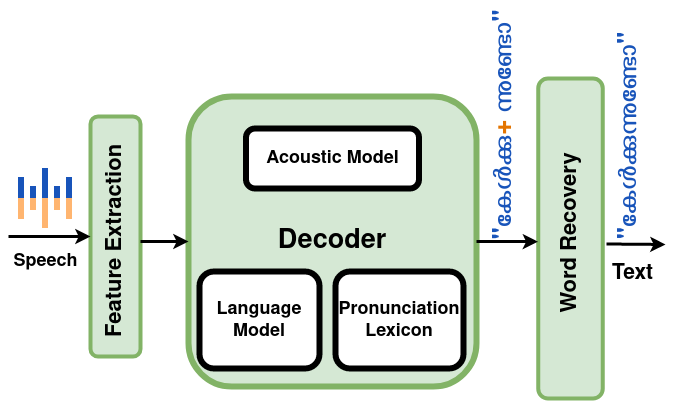
\includegraphics[width=0.8\linewidth]{ASR-subword.png}
    \caption{Block schematic representation of hybrid ASR system, with subword based language model and pronunciation lexicon}
    \label{fig:asr-subword}
\end{figure}

\gls{asr} is challenging for low resource languages in a
a morphologically complex setting \cite{besacier2014automatic}. Morphological
complexity is characterised by productive word formation by agglutination,
inflection, and compounding, leading to very long words with phonetic and
orthographic changes at morpheme boundaries \cite{baerman2015understanding}.
Malayalam language is known to have a high level of morphological complexity
than many other Indian and European languages in terms of \gls{ttr} and
\gls{ttgr}
\cite{bharadwaja2007statistical,manohar_quantitative_2020}. This creates a large
number of low frequency words and it is practically impossible to build a
pronunciation lexicon that covers all complex wordforms. Additionally, it
introduces the problem of data sparsity in language modelling
\cite{SMIT2021101158}.

% Low resource nature of the language with limited annotated audio corpus and underdeveloped computational linguistic tools for text processing makes acoustic and language modelling difficult in many ways. 
Deep learning based acoustic modelling improves speech recognition accuracy for
languages with abundant training data \cite{thai-etal-2020-fully}. Statistical GMM-HMM
or hybrid DNN-HMM methods are best suited for languages with limited labelled
audio \cite{georgescu2021performance}. When much more text data is available
than audio data, hybrid models are the preferred choice
\cite{bayerl2019comparison,aku2021specom}. Hybrid ASR models require explicit
pronunciation lexicons and language models as shown in Figure \ref{fig:hybridASR}.
Language modelling of morphologically complex languages can not achieve the
word sequence prediction capabilities of simple morphology languages
\cite{mielke-etal-2019-kind,10.1162/tacl00365}. Additionally, finite sized word
vocabulary of a pronunciation lexicon can not cover complex wordforms and loan
words that appear in a real world testing. As a result, there is a difficulty
in recovering words that are not in the lexicon. \cite{SMIT2021101158}.

% \begin{figure}[]
% 	\centering
% 	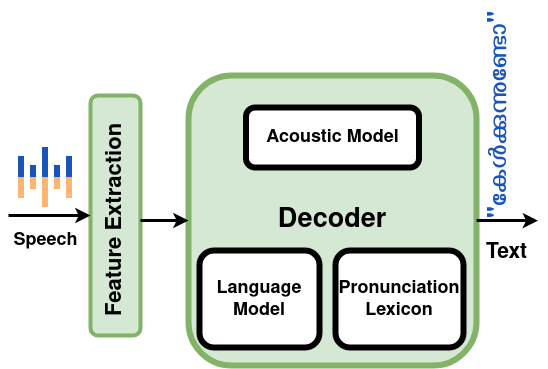
\includegraphics[width=0.9\linewidth, height=5cm]{ASR.png}
% 	\caption{Block schematic representation of Hybrid ASR system}
% 	\label{fig:asr}
% \end{figure}

The \gls{oov} rate is the proportion of words in a given speech
sample that are not present in the vocabulary of the ASR lexicon. OOV words can
not be recognised by the conventional word based ASR decoder. Large number of OOV words, and data sparsity
are the natural consequences of word based language models in ASR for
morphologically complex languages \cite{SMIT2021101158}. Segmenting words to appropriate subword
units before processing, and later reconstructing them to the whole words is a
viable approach to solve the issues of data sparsity and OOV rates. When
subword segments are used for language modelling, a dummy symbol is added to
identify the positions where the segments can be glued together to form words
\cite{smit17_interspeech}. When subwords replace words, the ASR vocabulary
contains morphemes, syllables, or other character sequences that together can
be used to create an unlimited number of words
\cite{creutz2007morph,sreeja-hybrid-2022}.
% However the ability of subword based LMs to recognise words unseen during training, has the the downside of producing invalid wordforms concatenating subword units. Additionally the search space for subword based ASR has to be guided by LMs with longer context information depending on the choice of subword unit \cite{SMIT2021101158}.

% Malayalam belongs to the family of Brahmic writing systems that is alphasyllabary in nature \cite{bri1999typology}. In this writing system, consonant–vowel sequences are written as a unit; each unit is based on a consonant letter, and the vowel notation is secondary. Though Malayalam script is largely phonemic in nature, there are some deviations like: (i) consonants with and without inherent vowel, (ii) consonant clusters with pronunciation different from the constituting consonants (iii) special symbol virama, that contextually chooses its function as a vowel killer or vowel inserter and (iv) graphemes being overloaded with non-native sounds in loan words \cite{kavya2022}. This implies acoustic features of these graphemes depends on the context of their appearance, which may be lost during subword segmentation that does not take into account these contexts.


% Subword segmentation has been employed in various natural language processing applications including statistical and neural machine translation \cite{sennrich-etal-2016-neural, kunchukuttan2016,banerjee-bhattacharyya-2018-meaningless}, speech recognition \cite{PASM2019, SMIT2021101158, sreeja-hybrid-2022, Creutz2007} and handwriting recognition \cite{singh2021online}.
Subword ASR decoder requires an additional module to reconstruct words from the
decoded subword units
% when subword based lexicons and language models are used in hybrid ASR, 
as shown in Figure \ref{fig:asr-subword}. Language modelling on subword segments in
ASR for morphologically complex languages has been extensively studied
\cite{creutz2007morph,HIRSIMAKI2006515,povey2006, Wang2020,zhou21d_interspeech} in
the context of hybrid ASR systems.  Subword segmentation based language modelling has been
proposed for applications in automatic speech recognition
\cite{SMIT2021101158,creutz2007morph,sreeja-hybrid-2022,adiga-etal-2021-automatic,PASM2019},
statistical machine translation \cite{kunchukuttan2016}, neural machine
translations \cite{sennrich-etal-2016-neural,kudo-2018-subword} and handwriting
recognition \cite{singh2021online}.


The reconstruction from subwords to words is facilitated by adding a dummy
marker symbol \cite{SMIT2021101158}. In the experiments we perform in this
work, we use continuity marker ``{\mal +}" to the right side of the subwords,
to indicate another subword has to follow it. In this approach, reconstruction
is straightforward, as the marker indicates the positions for joining the
following subword. The Table \ref{tab:marker} illustrates the usage of continuity
marker in our experiments.

%, by covering various other segmentation methods. 
% However we have not included the previously reported two step hybrid segmentation method that works on Malayalam-English code switched text \cite{sreeja-hybrid-2022}.
% In a previous study by Manohar  \cite{manohar2022nsurl}, it has been demonstrated that the use of subword segments is advantageous only on test datasets with medium to large OOV words. So we analyse the other impacts on medium OOV test dataset only.



% \subsection{Continuity Markers for Word Reconstruction}



\begin{table}[ht]

    \caption{Segmentation illustrating the usage of continuity marker symbol `{\mal +}'.}
    \label{tab:marker}
    \centering
    \begin{tabular}{ll}
        \hline \hline
        \textbf{Original Text}  &  \textbf{Segmented text}    \\ \hline

        {\mal അവൻ വള ഇടുകയില്ല}  & {\mal അ+ വൻ വള ഇടുക+ യില്ല } \\ \hline
    \end{tabular}
\end{table}

\section{Graphemic and Phonemic Pronunciation Lexicon}

For languages where space and punctuation marks act as delimiters between
words, segmenting raw text of the language into words is pretty
straightforward. However to segment text to subword units, there are data
driven as well as linguistically informed algorithms
\cite{besacier2014automatic,SMIT2021101158}. Morfessor
\cite{creutz2002unsupervised,creutz2007morph,virpioja2013morfessor}, \Acrfull{bpe} \cite{gage1994new,sennrich-etal-2016-neural} and Unigram
\cite{kudo-2018-subword} are a few data driven algorithms in popular use. These
algorithms do not ensure that subword segmentation happens at valid
pronunciation boundaries. This makes precise representation of its
pronunciation as a sequence of phonemes impossible.

\begin{table}[htpb]
    \caption{Phonemic Lexicon}
    \label{tab:phoenmiclexicon}
    \centering
    \begin{tabular}{cc}
        \hline  \hline
        \textbf{Word} & \textbf{Pronunciation} \\ \hline

        SOPHIA        & {\ipa s o ʊ f i ə}     \\ \hline
    \end{tabular}

\end{table}

For example if the word \textbf{SOPHIA} /{\ipa soʊfiə}/ is segmented as
\textbf{SOP+ HIA}, the pronunciation can not be segmented in a valid way. Then
what is viable is to represent each subword segment in the lexicon with its
pronunciation described as a grapheme sequence. Tables \ref{tab:phoenmiclexicon}
and \ref{tab:graphemiclexicon} indicate how these entries would be represented in a
phonemic and graphemic lexicon respectively. In this work, we use graphemic
lexicons and graphemes would be mapped to acoustic features during acoustic
model training. Subword based lexicon has the continuity marker ``{\mal +}"
indicating it will be followed by another subword segment to complete a word.

% These pronunciation units (phonemes or graphemes) would be mapped to acoustic features during acoustic model training.

\begin{table}[ht]

    \caption{Graphemic Lexicon}
    \label{tab:graphemiclexicon}
    \begin{center}

        \begin{tabular}{lr}

            \begin{tabular}{c|c}
                \hline  \hline
                \textbf{Word} & \textbf{Pronunciation} \\  \hline
                SOPHIA        & S O P H I A            \\
                & \\
                \hline
            \end{tabular}

             &

            \begin{tabular}{c|c}
                \hline  \hline
                \textbf{Subword} & \textbf{Pronunciation} \\  \hline
                SOP{\mal +}      & S O P                  \\
                HIA              & H I A                  \\
                \hline
            \end{tabular}

        \end{tabular}

    \end{center}
\end{table}

% BPE (segment by letter-sequence frequency)
% Morpheme like units using Morfessor(Segment by long letter-sequence frequency)

% (BPE and morpheme segmentation may happen at invalid pronunciation boundaries. So pronunciation of these segments can not be represented precisely as a sequence of phonemes.)

% Segmenting the text of a language to subword units can be carried out using language specific rule based approaches or language independent unsupervised approaches. Language independent unsupervised segmentation algorithms do not ensure words are split at valid pronunciation boundaries. In such cases acoustic modelling has to be done on graphemes, which are otherwise generally done on phonemes. 

In this work, we propose two linguistically motivated subword segmentation algorithms.  First one is a purely linguistic syllabification approach, tailored specifically for Malayalam. The second one is a hybrid subword segmentation algorithm, S-BPE,
combining linguistic syllabification rules with the data driven segmentation
method of BPE. We design our experiments to answer two related research
questions:
% In the algorithms we propose, segmentation happens only at valid pronunciation boundaries and hence pronunciation description can be done either with phonemes or with graphemes. We have designed our experiments to answer two related research questions focusing on Malayalam language:

\begin{enumerate}
    \item How does segmentation method affect the language modelling complexity in a
          morphologically complex setting?
          % \item Does linguistically informed segmentation at valid pronunciation boundaries improve ASR performance in a morphologically complex setting?
    \item How does the choice of segmentation strategy affect the ASR performance in
          terms of \gls{wer}, \gls{oov}-\gls{wer} and model memory requirement?

\end{enumerate}

Due to the low resource nature of Malayalam with limited audio training data
but comparatively higher amount of text data, we experiment on hybrid DNN-HMM
based ASR for Malayalam, where acoustic and language models are trained
separately \cite{bayerl2019comparison,aku2021specom}.

% \section{Key Contributions}

% This paper proposes a novel subword segmentation method for Malayalam text. We compare this methods with existing linguistically informed and data driven methods of subword segmentation and analyse their impact on hybrid DNN/HMM based ASR task. 
% % Additionally we compare the effect of grapheme based and phoneme based units in acoustic modelling in Malayalam ASR. 
% In the following sections we describe the related works, present the proposed algorithm, describe the experimental setup, analyse the results which lead to answers for the research questions posed in the earlier section. 

% \section*{Morphological complexity of Malayalam}

% Malayalam belongs to Dravidian language family that has high levels of morphological complexity 
% \begin{table}[ht]

% 	\caption{Complex morphological word formation in Malayalam }
% 	\label{morph-ml} 

% \centering
% \begin{tabular}{p{2.7cm} p{3cm}}
%  \bf Malayalam Word & \bf English Translation  \\ \hline

% {\mal പെട്ടിയിൽ}/{\ipa peʈʈijil}/& in the box  \\

% {\mal കുട്ടിയോട്} /{\ipa kuʈʈijoːʈ}/& to the child \\ 

% {\mal ആനക്കുട്ടി}/{\ipa aːnakkuʈʈi}/ & baby elephant  \\ 

% {\mal ആനക്കുട്ടികളോട്} /{\ipa aːn̪akkuʈʈikaɭoːʈ}/ & to the baby elephants \\ 

% {\mal ഉണർന്നിരിക്കണ്ട} /{\ipa uɳaɾn̪n̪iɾikkaɳʈa}/& do not stay awake \\ 

% {\mal പാടിക്കൊണ്ടിരിക്കും} /{\ipa paːʈikkoɳʈiɾikkum}/ & will be singing \\

% \end{tabular}

% \end{table}

% \section{Background and Related Works}

\section{Subword Segmentation Strategies -  A Review}
\label{segmentation-literature}

A language model estimates the likelihood of word or subword sequences to form
a valid sentence. To estimate these likelihood, the raw text of the language
has to be segmented into words or subwords. This section explains various
segmentation strategies proposed in literature. The suitability of subword
segmentation depends on the task (speech recognition, machine translation, text
prediction etc.) under consideration. Segmentation techniques that could be
adapted for Malayalam language are used in the ASR experiments performed in
this research work.

Orthographic syllable based segmentation of text was proposed by Kunchukuttan
et al. for statistical machine translation applications
\cite{kunchukuttan2016}. Splitting the tokens based on vowels and adjacent
consonants, named Vowel segmentation, was proposed by Adiga et al. and employed
in the context of Sanskrit speech recognition \cite{adiga-etal-2021-automatic}.
These two methods segment text to syllable-like units at valid pronunciation
boundaries.



% Vowels occur only at the beginning of a word (\texttt{<BoW>}). Syllables end in \textit{virama} only at end of words (\texttt{<EoW>}).  A syllable in Malayalam is structured in one of the following ways as indicated in Table \ref{syllablestructure}.

% \label{syllablestructuretable}
% \begin{figure}[ht]
% 	\centering
% 	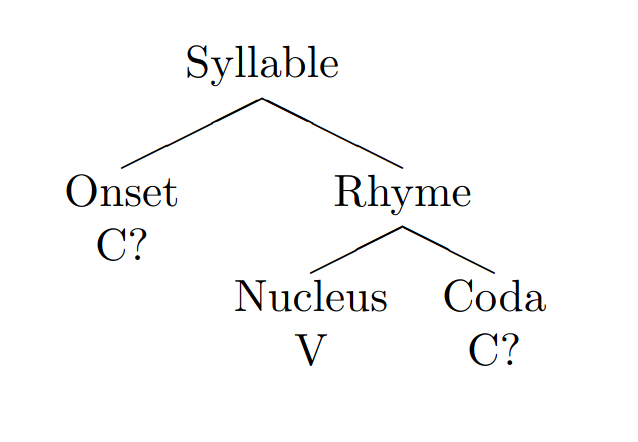
\includegraphics[width=0.6\linewidth]{syllable.png}
% 	\caption{Structure of a syllable. C - consonant /consonant cluster, V - vowel, ?- indicates optionality}
% 	% \Description{Syllable structure described as a tree}
% 	\label{syllable}
% \end{figure}

% A syllable  is typically composed of a mandatory vowel nucleus, along with optional consonants or consonant clusters in onset and coda posions. A syllable in Malayalam can be  a consonant or a conjunct, followed by an optional vowel sign. A standalone vowel is also a syllable, that occur only at word beginnings. Whenever a special consonant appears, it becomes the syllable ending consonant \cite{prabo2016}. 

Several approaches for segmenting Malayalam text to meaningful morpheme units
incorporating linguistic knowledge are reported in literature. But for the
reasons listed below, none of these could be used for the language modelling
task required for ASR. For Malayalam morphological segmentation, earlier
studies have used probabilistic, rule-based suffix-stripping, machine learning
and dictionary-based approaches \cite{rajeev2007suffix, rinju2013morphological,
    antony2012computational,abeera2010morphological}. The most recent deep learning
technique uses Romanised Malayalam text and require annotated data for training
\cite{dlmorph-mal-2018}. However, none of these research offers an API that can
be programmed to perform morphological segmentation for use in downstream
applications. The only tool with a programmable interface that works with
Malayalam script performs morphological analysis\footnote{Mlmorph:
    \url{https://pypi.org/project/mlmorph/}} and not morphological segmentation
\cite{thottingal2019finite}. For example we need the compound word {\mal
        ആനകൾ} {\ipa /aːnakaɭ/} to be segmented as {\mal ആന+ കൾ} {\ipa /aːna+/ /kaɭ/},
while its morphological analysis returns {\mal ആന}\texttt{<noun><plural>}.
Morphological analysis is not appropriate for an ASR task, as we expect to
piece together the original word from morpheme segments by concatenation. For
the ASR task, we therefore do not rely on any linguistically informed morpheme
segmentation in Malayalam.

The data driven segmentation methods are designed only based on word spellings
and do not have access to pronunciation information. It is therefore possible
for these algorithms to break a word sequence into units that do not imply
well-formed correspondence to phonetic units. \Gls{pasm} is an algorithm proposed to solve this issue by using a
pronunciation dictionary as an aligner to determine the positions for
segmentation \cite{PASM2019}. To perform this task, PASM needs a pronunciation
dictionary. It uses CMUDict to report the results on English language. But many
low resource languages do not have a ready to use pronunciation dictionary. In
the comparative analysis performed in this work, we use several segmentation
methods that breaks the pronunciation flow. So to be fair in the comparison, we
use only graphemic lexicons and not phonemic ones. In this scenario, PASM for
segmentation is not used.

% A rule based morphological analyser that works on native Malayalam script \cite{thottingal-2019-finite} provides morpheme sequences along with part-of-speech (POS) tags. But these morpheme segments show phonetic changes at morpheme boundaries. So pronunciation of these subwords could differ from what is actually spoken in the acoustic modelling coprus. Also the compound word can not be reconstructed by simple concatenation. For example the compound word {\mal ഇടുകയില്ല} /{\ipa iʈukajilla}/, constituted by the morphemes {\mal ഇടുക}{\ipa /iʈuka/}\texttt{<verb>} and {\mal ഇല്ല}{\ipa /illa/ }\texttt{<negation>}, has the character {\mal യ} {\ipa /j/} inserted at the boundary. 

For ASR applications in morphologically rich languages, a segmentation
technique that ensures rare subwords are included in the vocabulary was
proposed by Manghat et al. \cite{sreeja-hybrid-2022}. This is the first work
that uses subword based language modelling in Malayalam - English code switched
ASR. Since the algorithmic implementation is not publicly available, we have
not attempted its usage in the experiments in this work.

The segmentation techniques already reported in literature and that could be
adapted for Malayalam language and employed in the experiments reported in this
work are described in the following subsections.

\subsection{Word Segmentation}

In Malayalam, the technique of word segmentation is simple. After removing
punctuation, the raw text corpus is divided up by spaces.

% \subsubsection{Morpheme Segmentation - Using Linguistic Knowledge }

\subsection{Morpheme Segmentation - Using Morfessor}

Morfessor is a language independent, data driven method of subword
segmentation. The Morfessor baseline algorithm is based on minimum description
length principle \cite{creutz2002unsupervised}. It is an unsupervised technique
in which frequently occurring sub strings in several different word forms from
the raw training text corpus are proposed as morphs (or morpheme-like units)
and the words are then represented as a concatenation of morphs
\cite{creutz2007morph}. Its current version, Morfessor2.0, has a Python interface
that may be customised and it supports annotated training data as well
\cite{virpioja2013morfessor}. The Morfessor method guarantees neither
segmentation at appropriate pronunciation boundaries nor segmentation into
meaningful units.

\subsection{BPE Segmentation}

\gls{bpe} is a data driven algorithm that determines the optimal set of subword
tokens through an iterative process. It was originally proposed as a data
compression algorithm \cite{gage1994new}. BPE algorithm splits the training
data into characters and create an initial vocabulary. During further
iterations, the most frequent character bigrams are determined, merged into a
single token and added to the vocabulary. The process is continued until a
desired number of merge operations are performed. The final vocabulary size is
the sum of initial vocabulary and the number of merge operations, which is a
hyper-parameter. The subword tokens in the learnt vocabulary are later used to
segment any text. BPE ensures that the most common words are represented in the
pronunciation dictionary as a single token while the rare words are broken down
into two or more subword segments \cite{sennrich-etal-2016-neural}. BPE
segmentation algorithm available in \texttt{subword-nmt} python library is used
in the experiments described in this work\footnote{subword-nmt:
    \url{https://pypi.org/project/subword-nmt/}}.
% This segmentation algorithm is published as an open source python library. %licensed for modification and reuse.

\subsection{Unigram  Segmentation}

Unigram segmentation \cite{kudo-2018-subword} is another language independent
segmentation algorithm. It makes the assumption that the subwords of the
sentence are independent of one another. The vocabulary of desired size is
built from a heuristically large vocabulary by retaining only $\eta \%$ (say
$\eta =80$) of the subwords in each iteration, and discards the rest. The top
$80\%$ of subwords are obtained by ranking all subwords according to the
likelihood reduction on removing it from the vocabulary. The most probable
segmentation of an input sentence is determined by the Viterbi algorithm. The
Unigram segmentation algorithm is available in the open source python library,
\texttt{sentencepiece}\footnote{sentencepiece:
    \url{https://pypi.org/project/sentencepiece/}}, which is used in the
experiments performed in this work.
% Text segmentation using this library, does not always happen at valid pronunciation boundaries.

% \subsubsection{M-BPE Segmentation}
% M-BPE, an approach combining two data driven techniques, Morfessor and BPE, was proposed by Banerjee et al. to perform subword segmentation for neural machine translation  \cite{banerjee-bhattacharyya-2018-meaningless}. M-BPE segmentation does not ensure splitting  at valid pronunciation boundaries.

% \subsubsection{PASM}

% \subsubsection{Hybrid Segmentation}

% as shown in Figure \ref{syllable}. 
% The sequence of characters and signs that constitute a valid orthographic syllable in Malayalam can be summarised as:
% \begin{enumerate}
% 	\item \textbf{Type 1:} Every independent vowel occurring at word beginning is a syllable. It may optionally be followed by a special consonant.

% 	      eg:  {\mal അ} {\ipa /a/} (V) in {\mal അമ്മ} {\ipa /a.mma/} (\textit{mother}),	

%       {\mal അം} {\ipa /am/} (VC) in {\mal അംബുജം} {\ipa /am.bu.ɟam/} (\textit{lotus}),

% 	\item \textbf{Type 2:} Every consonant with or without vowel sign at end is a syllable. It may optionally be followed by a special consonant.

% 	      eg: {\mal ക} {\ipa /ka/} (CV) in {\mal കളി} {\ipa /ka.ɭi/} (\textit{game}),

% 	      {\mal കി} {\ipa /ki/ }(CV) in {\mal കിളി} {\ipa /ki.ɭi/} (\textit{bird}),

% {\mal വൻ} {\ipa /ʋan/} (CVC) in {\mal അവൻ}  {\ipa /a.ʋan/ }(\textit{he})

% 	\item \textbf{Type 3:} Every consonant cluster with or without vowel sign at end is a syllable. It may optionally be followed by a special consonant.

% 	    eg:   {\mal സ്ത} {\ipa /st̪a/} (CCV) in {\mal പുസ്തകം} {\ipa /pu.st̪a.kam/} (\textit{book}),

% 	      {\mal ഷ്ടി} {\ipa /ʂʈi/} (CCV) in {\mal ഇഷ്ടിക} {\ipa /i.ʂʈi.ka/} (\textit{brick}),

%           	      {\mal സ്ത്രം} {\ipa /st̪ram/} (CCCVC) in {\mal അസ്ത്രം} {\ipa /a.st̪ram/} (\textit{arrow})
% \item
%  \textbf{Type 4:} A consonant or consonant cluster followed by a \textit{virama} if and only if at word ends, is a syllable.  The \textit{virama} can optionally be preceded by the u-vowel sign {\mal ു}. In this scenario, the vowel sound is schwa {\ipa /ə/}, which does not have an explicit vowel grapheme in Malayalam.
% 	       eg:  {\mal ന്} {\ipa /nə/} (CV) in {\mal അവന്} {\ipa /a ʋa nə/} (\textit{him}),

% 	      {\mal ട്ട്} {\ipa /ʈʈə/} (CCV) in {\mal പട്ട്} {\ipa /pa ʈʈə/} (\textit{silk}),

% 	      {\mal ട്ടു്} {\ipa /ʈʈə/} (CCV) in {\mal പട്ടു്} {\ipa /pa ʈʈə/} (\textit{silk}),

% 	      \end{enumerate}

% \begin{table}[ht]
%     \caption{ Syllable structure in Malayalam with examples}
%    \label{syllablestructuretable} 
%         \centering
%   \begin{threeparttable}[b]

%   \begin{tabular}{lll}
%     \hline \hline
%     \textbf{Type} & \textbf{Syllable Structure}      & \textbf{Example}                \\
%     \hline
% \multirow{2}{*}{1}  & \texttt{<BoW>}\tnote{*}+Vowel           & {\mal അ} {\ipa /a/}   \\
%    & \texttt{<BoW>} +Vowel+Special Consonant      & {\mal അം} {\ipa /am/} \\
%     \hline
%   \multirow{3}{*}{2}   & Consonant         & {\mal ക} {\ipa /ka/} \\
%     &Consonant+Special Consonant     & {\mal കൾ} {\ipa /kaɭ/}\\
%     &Consonant+Vowel sign+Special Consonant& {\mal കിം} {\ipa /kim/ } \\
%     \hline
%     \multirow{3}{*}{3} & Conjunct        & {\mal സ്ത്ര} {\ipa /stra/}\\
%    & Conjunct+Special Consonant & {\mal സ്ത്രം} {\ipa /st̪ra/}\\
%     & Conjunct+Vowel sign+Special Consonant& {\mal സ്ക്രീം} {\ipa /skriːm/}\\
%     \hline
%   \multirow{2}{*}{4} & Consonant+  \textit{virama} + \texttt{<EoW>}\tnote{\#}
%  & {\mal ക്} {\ipa /kə/} \\
%    & Conjunct + {\mal ു} + \textit{virama} +\texttt{<EoW>} & {\mal ട്ട്} {\ipa /ʈʈə/} \\
%     \hline
%   \end{tabular}
%       \begin{tablenotes}
%       \item [*] Beginning of Word
%     \item [\#] End of Word
%      \end{tablenotes}
%     \end{threeparttable}
% \end{table}

% \begin{figure*}[ht]
% 	\centering
% 	\includegraphics[width=0.9\textwidth]{syllable-drawio.png}
% 	\caption{Syllabification FST, performing syllabification on the words {\mal അവൾ} and {\mal അവൻ}. }
% 	\label{sylfst}
% \end{figure*}

% These four types of syllable structures in Malayalam are tabulated in Table \ref{syllablestructuretable}.
% The algorithm to parse the Malayalam text and insert syllable boundary tags at appropriate positions is presented in Algorithm \ref{syllabifier-algorithm} \cite{kavya2022}. 

% A group of characters that do not fit into one of the categories described in this section cannot be combined to form a syllable. A vowel sign following an independent vowel ({\mal അി}), a word beginning with a virama ({\mal ്ക്കം}), an independent vowel after a consonant ({\mal കിഅ}) etc. are  examples of invalid character sequences.

% The text to be syllabified is cleaned up to remove punctuation and foreign scripts and is split to word tokens, prior to applying syllabification algorithm. The sequence of characters that constitute a syllable are identified and markers - \texttt{<BoS>}, \texttt{<EoS>} - are inserted at appropriate positions to indicate the beginning and end of the syllables respectively. If the token passed to the syllabifier is {\mal അവൻ}, it returns the syllabified string  \texttt{<BoS>}{\mal അ}\texttt{<EoS><BoS>}{\mal വൻ}\texttt{<EoS>}.  The string to string mapping rules are implemented as FSTs using SFST toolkit \cite{schmid2005programming}. Figure \ref{sylfst} illustrates the state transitions and the insertion of markers in the syllabifier FST when input tokens passed are: {\mal വള} and {\mal അവൻ}. Note that {\ipa ε} indicate the empty transition string. The boundary tags will be replaced by continuity markers `{\mal +}' at appropriate positions before employing them in language modelling and pronunciation lexicons.

\section{Proposed Subword Segmentation Algorithms for ASR}
\label{sec:sbpe}
In this section, we present the details of our proposed subword segmentation algorithms. The first one is the FST based syllabification algorithm and the other is the hybrid algorithm combines the data driven approach of BPE with linguistic information about syllables.

% Any language that could be syllabified can use this algorithm to segment text.

% \subsection{FST based Syllabification Algorithm}

% Syllables are well defined orthographically  in the Malayalam linguistic literature and grammar textbooks \cite{asher1997,prabo2016,mohanan1989syllable}. Syllables serve as a standalone pronunciation unit and can be described as a sequence of phonemes in a pronunciation dictionary. This makes them an appropriate choice for subword unit in ASR. 


\subsection{Syllable Segmentation}
\label{sec:ch-openvocab-syllabification}

To performs segmentation that aligns with the Malayalam script, it is important
to analyse the nature of grapheme inventory of Malayalam. The graphemes in
Malayalam script are classified as:
% \begin{enumerate}
%     \item Vowels
%     \item Vowel signs %($V_s$)
%     \item Regular consonants
%     \item Special consonants %($C_s$)
%     : \textit{anuswara}, \textit{visarga}, \textit{chillu}, \textit{dotreph}
%     \item Multi-functional character: \textit{virama}
% \end{enumerate}
(i) Vowels, (ii) Vowel signs, (iii) Regular Consonants, (iv) Special consonants : \textit{anuswara}, \textit{visarga} and \textit{chillu}, and (v) Multi-functional character: \textit{virama}. Vowel graphemes occur only at word beginnings. Regular consonants inherently have the vowel /{\ipa a}/ present in them. Vowel sounds at positions other than word beginnings are represented by vowel signs. Vowel signs modify the inherent vowel sound of the consonants. A consonant cluster, also known as a conjunct, in Malayalam is a sequence of consonants separated by \textit{virama} in between, where \textit{virama} kills the inherent vowel from the preceding consonant \cite{asher1997}. \textit{Chillus} are special consonants that do not have inherent vowel associated with them. The characteristics of other special consonants and \textit{virama} are marked in Table \ref{tab:specialsigns}. The syllabification process will make use of these linguistic rules.

\begin{table}[htpb]
    \caption{Special consonants and Virama sign in Malayalam}
    \label{tab:specialsigns}
    \centering
    \begin{tabular}{ll}
        \hline \hline
        \textbf{Character} & \textbf{Properties}                    \\ \hline
        \textit{Anuswara}  & Represents /m/ at syllable ends        \\
        \textit{Visarga}   & Introduces aspirated glottal stop      \\
        \textit{Chillu }   & Dead consonants with no inherent vowel \\
        \textit{Virama}    & Kills Inherent vowel in conjuncts      \\
                           &  and inserts schwa at  word ends.           \\

        \hline \hline
    \end{tabular}
\end{table}

% There are knowledge based approaches for subword segmentation where language specific rules are incorporated. 
A syllabification algorithm tailored for Malayalam script using finite state
transducers has been introduced in Chapter \ref{ch:Mlphon}. The linguistic rules
for syllable segmentation has been computationally implemented as in Algorithm
\ref{syllabifier-algorithm} and made available as part of the \texttt{Mlphon}
Python library\footnote{\url{https://pypi.org/project/mlphon/}}. We use
Mlphon, to perform syllable segmentation. This results in a variable
length subword segments where each segment is a syllable with valid pronunciation.

\begin{algorithm*}[ht]
    \caption{FST based Syllabification Algorithm}\label{syllabifier-algorithm}
    \begin{algorithmic}[1]
        \Procedure{Syllable boundary tagging}{}
        \State {\ipa c\_v} $\gets$ {\ipa consonant + virama}
        \State {\ipa Type 1} $\gets$ {\ipa <BoW> + vowel+[anuswara, visarga, chillu] ?}  \Comment{? indicates optionality}
        \State {\ipa Type 2} $\gets$ {\ipa consonant + vowelsign ? + [anuswara, visarga, chillu]?}
        \State {\ipa Type 3} $\gets$ {\ipa c\_v * + C} \Comment{* indicates one or more occurence}
        \State {\ipa Type 4} $\gets$ {\ipa c\_v ? + consonant + {\mal ു}? + virama + <EoW>}
        \State {\ipa syllable} $\gets$ {\ipa[Type 1, Type 2, Type 3, Type 4]} \Comment{Defines a syllable}
        \State \texttt{SyllableBoundaryTagger}: {\ipa <BoS>+ syllable +  <EoS>} $\gets$ {\ipa syllable}
        \EndProcedure
    \end{algorithmic}
\end{algorithm*}
% \subsubsection{Malayalam Syllabifier}






\subsection{S-BPE Algorithm}

\gls{sbpe} is a hybrid algorithm that takes into account syllables as irreducible
units in the same way that BPE takes into account characters. \gls{sbpe} algorithm
needs to learn the syllable sequence frequencies from a training corpus, before
it can be applied to segment words. During training, it creates a symbol
vocabulary of most frequent syllable sequences. During segmentation, the
algorithm compares the text with the symbol vocabulary file and segments the
words into subwords that are most frequent sequence of syllables. The
algorithmic implementation has been adapted from the original BPE algorithm in
\texttt{subword-nmt} python library, and made available under MIT License
\footnote{{\url{https://github.com/kavyamanohar/subword-syl-bpe-ml/tree/sbpe}}}.

\subsubsection{Training}
To begin with, the words in the S-BPE training corpus are syllabified using the
Algorithm \ref{syllabifier-algorithm}. A symbol vocabulary, $V$ is created by
populating it with the unique syllables. The words in the training corpus is
searched to determine the most frequent symbol bigram and that bigram is then
merged and added as a new entry to the symbol vocabulary. All the occurrences
of this bigram will be replaced in the training corpus using the newly merged
symbol bigram. This step is repeated for a desired number of times, $k$ as
described in Algorithm \ref{sbpe-algorithm}. The number of merge operations is
set to $k=10000$, in our experiments.

\begin{algorithm}[ht]
    \caption{S-BPE Training Algorithm}\label{sbpe-algorithm}
    \begin{algorithmic}[1]
        \Require{Set of strings D, Number of merges k}
        \Procedure{S-BPE}{D, k}
        \State{{\ipa Vocab} $\gets$ {\ipa All unique syllables in D}}  %\Comment{Syllabification done using Algorithm \ref{syllabifier-algorithm}}
        \State { ${merge\_counter}$ = 0}
        \While{ $merge\_counter$ < k} \Comment{Merge frequent bigrams}
        \State{$S_L$, $S_R$ $\gets$ {\ipa Most frequent bigram in D}}
        \State{$S_{new}$ $\gets$ $S_L$+$S_R$} \Comment{Merge most frequent symbols}
        \State{{\ipa Vocab} $\gets$ Vocab + $S_{new}$}
        \State{{\ipa Replace each occurrence of $S_L$, $S_R$ with $S_{new}$}
            \State{$merge\_counter$ = $merge\_counter$ + 1}
        }
        \EndWhile
        \EndProcedure
    \end{algorithmic}
\end{algorithm}

% S-BPE is different from the M-BPE approach discussed in \cite{banerjee-bhattacharyya-2018-meaningless}. M-BPE algorithm starts with segmenting the training corpus to morphemes using Morfessor \cite{virpioja2013morfessor}. Now character lever BPE is applied to these morphemes to further segment it. 

\subsubsection{Segmentation}

First, the text to be segmented is syllabified using Algorithm
\ref{syllabifier-algorithm}. Then every instance of the syllable sequence
$S_L$, $S_R$ in the corpus to be segmented is replaced with $S_{new}$, in the
order in which those symbols were learnt and added to the vocabulary, {\ipa Vocab}. S-BPE
ensures that the most common words are represented in the vocabulary as a
single symbol while the rare words are broken down into two or more subword
segments while guaranteeing each segment has a valid pronunciation.

This entire process effectively combines the knowledge based syllabification
with the data driven BPE. The syllabification algorithm is tailored for
Malayalam script. However S-BPE algorithm can be extended to any language that
can be syllabified.

% \section{Methodology}

% This section describes our approach towards designing the experiments to answer our research questions. We use Kaldi toolkit for our hybrid DNN/HMM experiments\footnote{\url{https://github.com/kaldi-asr/kaldi}}. 

% \subsection{Graphemic Pronunciation Lexicon}

% Multiple graphemes can have same pronunciation. This may affect the acoustic modelling capability by pointing two different symbols to be mapped to similar acoustic features. However phonemic lexicon built using a good grapheme to phoneme converter takes care of this situation and ensures representation of identical speech features of the language with the same phoneme. Mlphon python package is used to create the phonemic lexicon in our experiments\footnote{\url{https://pypi.org/project/mlphon/}}.

% \begin{table}[ht]
%     \caption{Segmentation strategies and associated pronunciation lexicon types. {\tick ✓} indicates the usage of the lexicon in that column }
%     \label{graphemicorphonemic}
%     \centering
%     \begin{tabular}{lcc}
%     \hline \hline
%       \textbf{Segmentation} & \textbf{Graphemic Lexicon} & \textbf{Phonemic Lexicon}\\ \hline
%         Word &{\tick ✓} &{\tick ✓} \\
%         BPE & {\tick ✓} & {\tick -}\\
%         Unigram & {\tick ✓} & {\tick -}\\
%         Morfessor & {\tick ✓}& {\tick -}\\
%         Syllable &{\tick ✓} & {\tick ✓}\\
%         S-BPE &{\tick ✓} & {\tick ✓}\\ \hline
%     \end{tabular}

% \end{table}

% We develop both graphemic and phonemic lexicons and incorporate them into our ASR model to address the research question regarding the selection of pronunciation unit (phonemes or graphemes), on its capability to better capture acoustic modelling information. Graphemic lexicons are created for each segmentation method under consideration. For segmentation based on words, syllables, and S-BPE, phonemic lexicons are also created as described in Table \ref{graphemicorphonemic}. We evaluate the graphemic and phonemic lexicons for these segmentation strategies in terms of final word error rate (WER). 

% The WER of an ASR decoder is largely influenced by the word or subword sequence knowledge of the LM, apart from what is inferred from the acoustic model. 
% Being a hybrid system composed of three different components, the WER depends not only on choice of pronunciation unit, but also on the word sequence knowledge incorporated into the system through an LM \cite{2019_latvian_graphemephoneme}. As a natural outcome, the reported results would only be indicative of the efficacy of selecting the investigated pronunciation unit when using ASR systems for word recovery. This need not imply that they are effective in a phonemic transcription of speech in the absence of word level language modelling data.

% \subsection{Lexicon Size and OOV Rate}
% \label{wordlecions}

% To study the impact of lexicon size on OOV rate and corresponding changes in final WER, we expand $PL1_{word}$.

% New words are added to the lexicon based on their frequencies in the language model training corpus. Details of the language model training corpus is given in section \ref{datasets}. When words in the LM training corpus is ranked in the order of their frequencies, we obtain a word frequency profile as shown in Figure \ref{rankplot}. 

% \begin{figure}[ht]
%     \centering
%     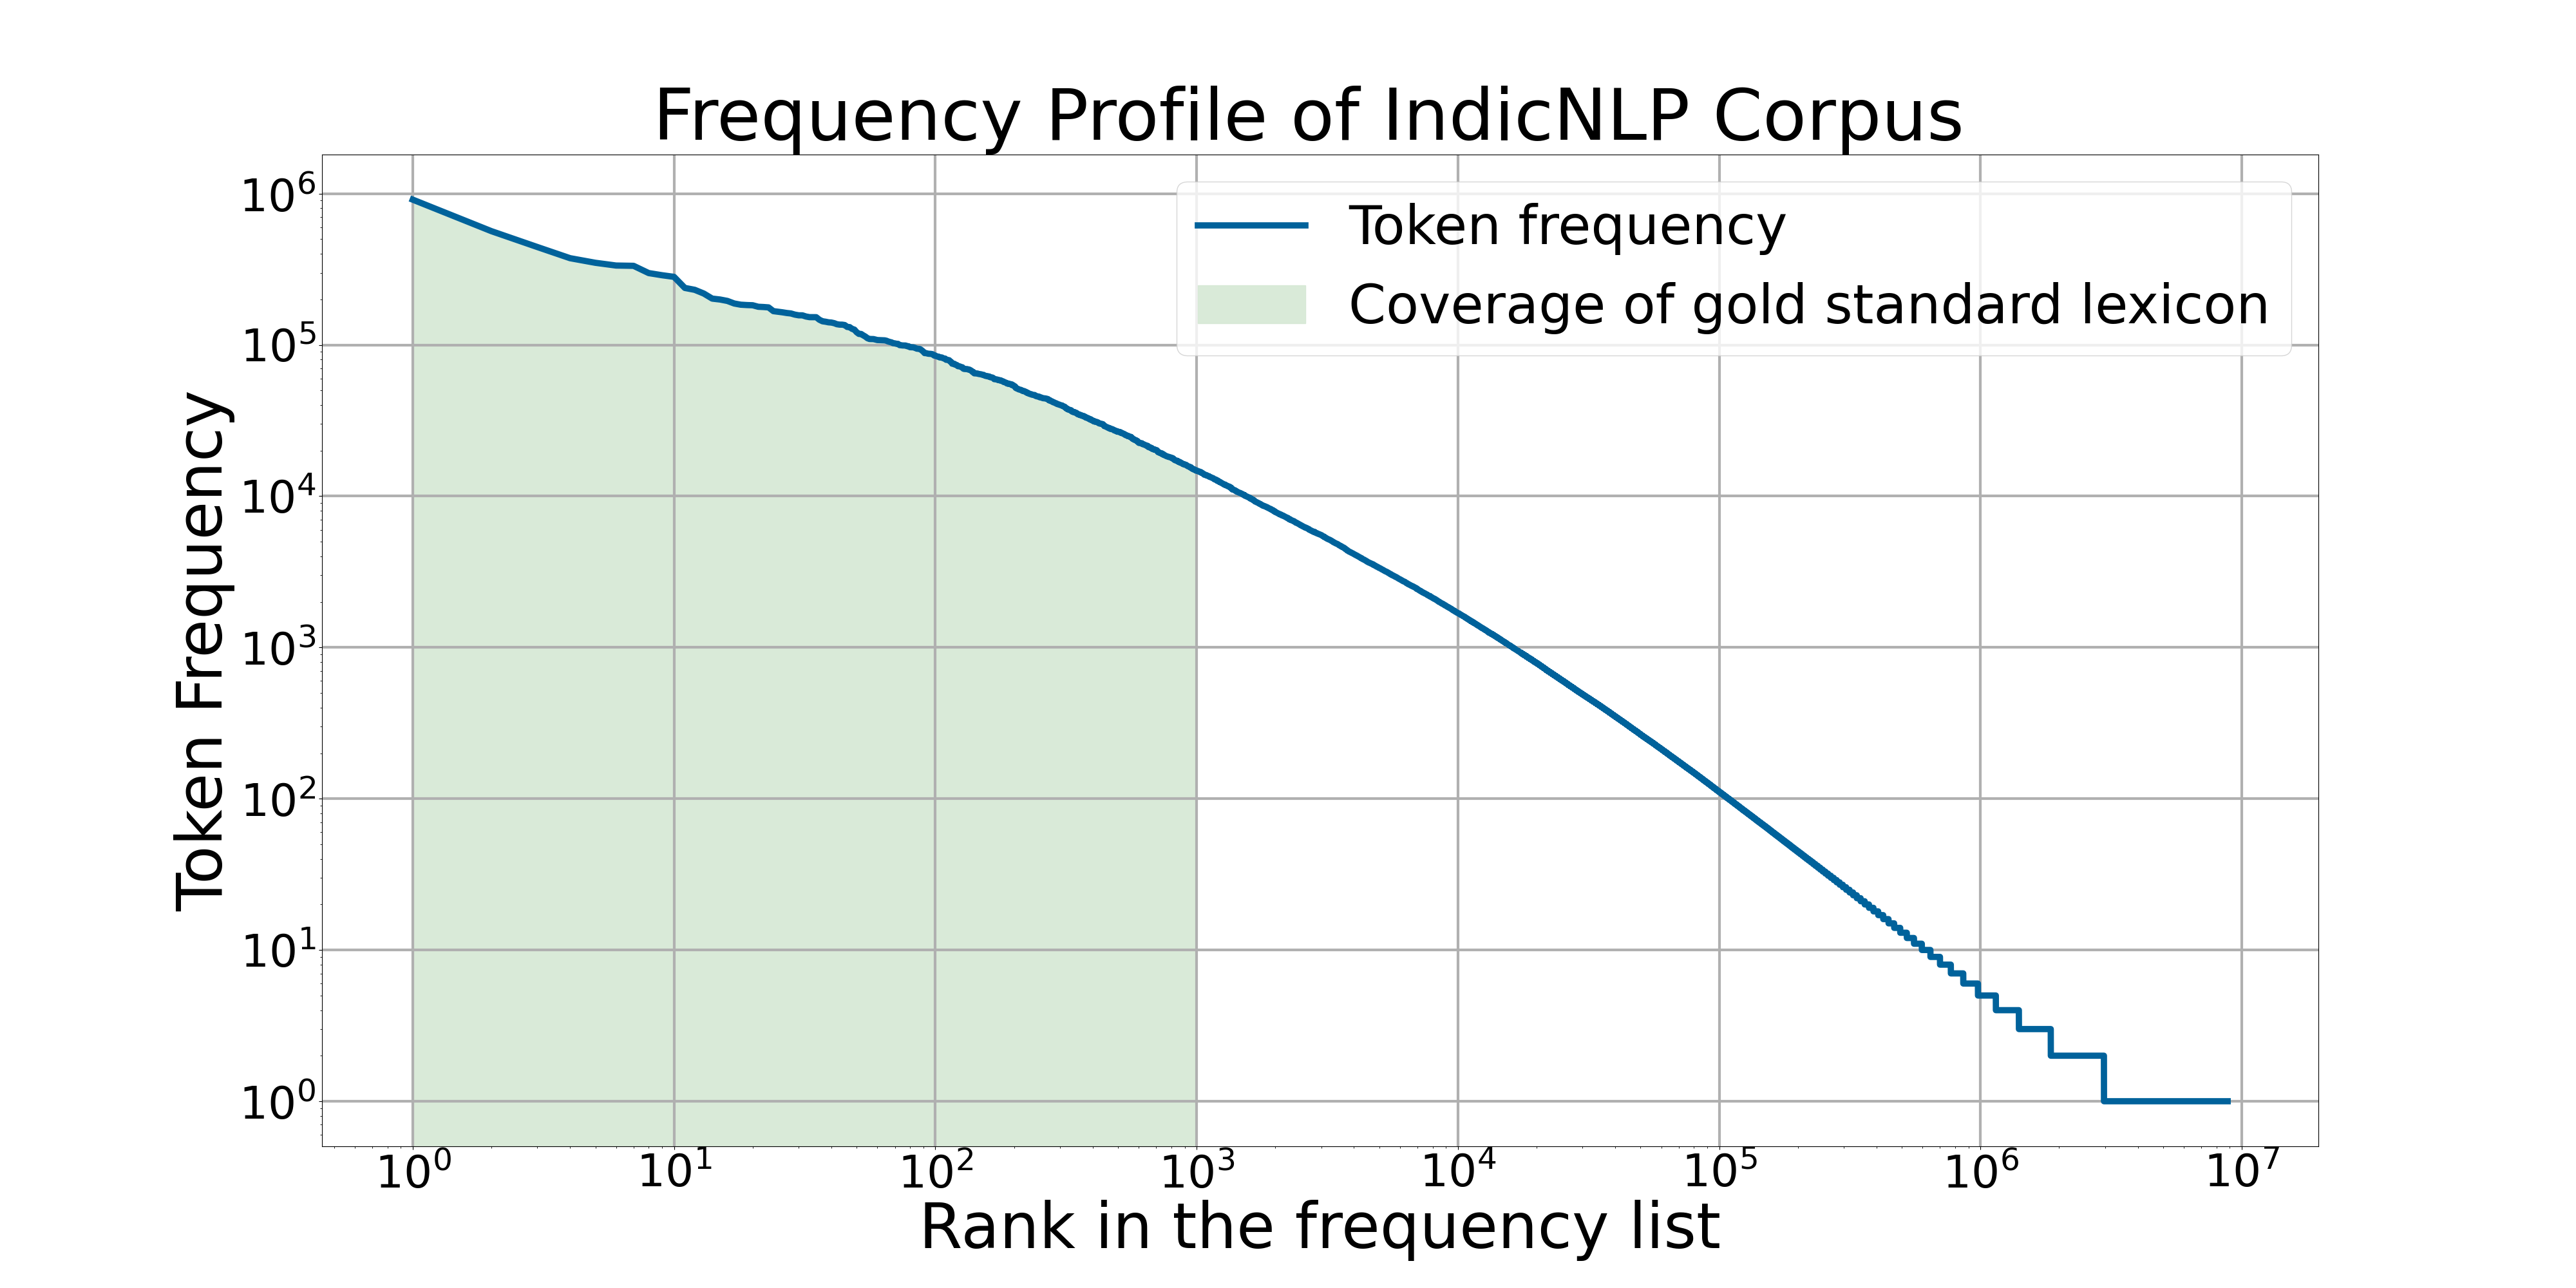
\includegraphics[width=\linewidth]{rank.png}
%     \caption{Word frequency profile of the text corpus for language modelling. The axes are on logarithmic scale.}
%     \label{rankplot}
% \end{figure}

% It can be seen that a huge portion of the corpus is covered by filling the pronunciation lexicon with high frequency words. We add words with at least 5, 4, and 3 frequencies to $PL1_{word}$ to obtain the pronunciation lexicons $PL2_{word}$, $PL3_{word}$ and $PL4_{word}$ respectively. Percentage of OOV words in different test datasets decreases with increase in vocabulary size, as indicated in  Table \ref{lexiconsize}. Test datasets are described in Section \ref{datasets}.

% \begin{table}[ht]
%   \caption{Comparison of word level OOV rates (\%) of test datasets, with word lexicon sizes}
%   \label{lexiconsize}
%   \begin{tabular}{c|c|ccc}
%   \hline \hline
% \textbf {Word Lexicon} & \textbf {Size} & \multicolumn{3}{@{}c@{}}{OOV Rate (\%)}\\ 
%                         &               & T1 & T2 & T3 \\
% \hline 
%  $PL1_{word}$& 	25604& 6.0  &    27.8 & 58.8 \\
%  $PL2_{word}$  & 53240 &   1.7  &    16.5  &   47.9\\
%  $PL3_{word}$  & 62483 &   1.6   &   15.7  &   46.9\\
%  $PL4_{word}$ & 79950 &   1.4    &  14.2   &  44.0 \\ \hline

%  \end{tabular}
% \end{table}

% Depending on the segmentation strategy, the created lexicon may be graphemic, phonemic or both.

\section{Experimental Setup}
\label{expsetup}

This section presents the details of our experiments\footnote{The Kaldi
    Experimental Setup:
    \url{https://gitlab.com/kavyamanohar/ml-subword-asr/-/tree/master/}}. We begin
with a description of the datasets followed by a discussion on building components for hybrid ASR system. We will describe in detail about the segmentation of the text corpus
for language modelling, creation of segmented pronunciation lexicons and the
process of acoustic modelling.

\subsection{Datasets}


We rely on publicly available open licensed read speech datasets
\cite{baby2016resources,he-etal-2020-open} for Malayalam. Every audio recording
in the dataset is associated with a textual transcript in Malayalam script. We
divide the available speech into train and test datasets, ensuring
non-overlapping speakers and speech transcripts.
%,prahallad2012iiit,smcspeech} 
% The first two rows in Table  represents the acoustic model training datasets while the next three rows represents the datasets used for testing the ASR model.
 The train datasets described in Table \ref{tab:speechdatasets} are combined to
get 1125 minutes of audio for acoustic modelling. The training dataset is same as that of the experiment described in chapter \ref{ch:lvcsr}. Since the focus of this chapter is on the usage of open vocabulary ASR to recover OOV words, we have not used the test dataset with fewer than 1\% OOV words.

\begin{table}[htpb]
    \caption{Details of Speech data sets used in our experiments. }
    \label{tab:speechdatasets-subword}
    \centering
    \begin{tabular}{clrrr}
        \hline \hline
        \textbf{Name} & \textbf{Corpus}                                     & \textbf{\#Speakers} & \textbf{\#Utterances} & \textbf{Duration} \\
                      &                                                     &                     &                       & (minutes)         \\
        \hline
        1             & Indic TTS, IITM \cite{baby2016resources}- Train     & $2$                   & $8601$                  & $838$               \\
        2             & Open SLR Malayalam \cite{he-etal-2020-open} - Train & $37$                  & $3346$                  & $287$               \\
        T1            & Open SLR Malayalam \cite{he-etal-2020-open} - Test  & $7$                   & $679$                   & $48$                \\
        % T2            & Festvox IIITH \cite{prahallad2012iiit} - Test       & 1                   & 1000                  & 98                \\
        % T3&MSC \cite{smcspeech}   -Test                             & 75                        &1541                       & 98                       & Read, Conversational & Natural, Noisy \\

        \hline

    \end{tabular}

\end{table}

% The testing datasets are retained without combining, so that we can separately evaluate the ASR model on these datsets with different OOV rates.

To create the language model, we use the sentences from the speech transcripts
and combine it with the curated collection of text corpus published by SMC
\cite{smctext}. From this, every sentence that appeared in our test dataset is
explicitly removed to prevent overfitting. The resulting text corpus contains
205k unique sentences, 1325k word types, and 356k unique word tokens.

\subsection{Hybrid ASR components}

The hybrid ASR decoder consists of three modules as described in Figure
\ref{fig:hybridASR}. The functions of these modules are listed below:

\begin{enumerate}
    \item The acoustic model predicts the posterior likelihood $Pr(X|Q)$ of  \gls{cd} tied phone HMM states $Q = {Q_0, Q_1, ...Q_K }$ given the
    acoustic feature vectors ${X} = {X_0 , X_1, ..., X_N }$. Modern acoustic
          models are usually implemented with deep neural networks. Deep neural network
          training relies on the frame level alignment of audio and phoneme labels
          obtained from a previously trained GMM-HMM acoustic model
          \cite{zelasko2022phoneticinventories}.

    \item The pronunciation lexicon maps words into sequence of phonemes. The acoustic
          model training module would need to look up the pronunciation lexicon to
          convert the word-level transcripts into phoneme sequences.

    \item The language model predicts the conditional likelihood $Pr(w_{i+1}|w_0 , w_1 , ...w_i )$ of the next word $w_{i+1}$ given the previous words.
\end{enumerate}

All these components are composed into a weighted finite-state transducer
framework \cite{MOHRI200269} and the most likely word sequence is retrieved
using graph search methods. This word based system would serve as the baseline
for our experiments.



Subword based ASR, as shown in Figure \ref{fig:asr-subword} is very much like word
based ASR system, except that (i) the language model represents the conditional
probability of subword sequences, instead of words and (ii) the pronunciation
lexicon is composed of subword segments. The word boundary marker is chosen so
that the predicted subword segments can be easily concatenated to form words.
We use the the segmentation methods described in \ref{segmentation-literature}
and \ref{sec:sbpe}, and compare them with the standard word-based ASR to answer
the research questions. The creation of segmented text corpus for subword
language model training and the creation of segmented pronunciation lexicons
are explained in the following subsections.

% To create the language model, we use sentences from the speech transcripts and curated collection of text corpus published by SMC \cite{smctext}. We explicitly remove every sentence that appeared in our test audio transcripts.

\subsection{Creating Segmented Text Corpora}

% about the best segmentation strategy for the morphologically complex Malayalam language.

% \begin{enumerate}
%     \item BPE Segments \cite{sennrich-etal-2016-neural}
%     \item Morfessor Segments \cite{virpioja2013morfessor}
%     \item Unigram Segments \cite{kudo-2018-subword}
%     \item Syllable Segments \cite{kavya2022}
%     \item Proposed S-BPE Segments
% \end{enumerate}

This section explains the text corpus segmentation procedure. Morfessor, BPE
and Unigram are data driven segmentation algorithms while S-BPE is a hybrid one
that additionally relies on linguistic knowledge. We use a subset of the text
corpus (7.5k sentences) to train the data driven and hybrid models.

\begin{enumerate}

    \item Words are separated by spaces in the text corpus and are easily segmented.

    \item

          Using the default settings with Morfessor 2.0 \cite{virpioja2013morfessor} we
          trained Morfessor on the training set and applied it to create morpheme
          segmented text corpus.

    \item
          BPE \cite{sennrich-etal-2016-neural} learns the vocabulary from the training
          dataset. The initial vocabulary is formed by the Malayalam characters in the
          training dataset. The number of merge operations is set to 10000. This results
          in a BPE model which is used to obtain the BPE segmented text corpus.
    \item Unigram \cite{kudo-2018-subword} model is trained by the \texttt{sentence
              piece} library using the training dataset with a vocabulary of 15000. The
          trained Unigram model is used to get the Unigram segmented text corpus.

    \item

          Being a rule based algorithm, syllabifier requires no training. Algorithm
          \ref{syllabifier-algorithm} is directly applied on the text corpus to obtain
          syllable segmented corpus.

    \item

          S-BPE model is trained using the Algorithm \ref{sbpe-algorithm} so that the
          vocabulary is learnt. The initial vocabulary is formed by the Malayalam
          syllables present in the training dataset. The number of merge operations is
          set to 10000. This results in a model which is used to obtain S-BPE segmented
          text corpus.

\end{enumerate}

Samples of text segmented using these methods are presented in Table
\ref{tab:segmentationexamples}.

\begin{table}[ht]
    \caption{Examples for different segmentation strategies. Space is used as delimiter between segments.}
    \label{tab:segmentationexamples}
    \centering
    \begin{tabular}{llc}
        \hline \hline
        \textbf{Method} & \textbf{Example}                 & \textbf{Segment count} \\
        \hline
        Word            & {\mal അവൻ വള ഇടുകയില്ല}             & 3                      \\
        & {\ipa /aʋan ʋaɭa iʈukajilla/} & \\
       Morfessor       & {\mal അവ+ ൻ വള ഇട+ ുക+ യില്ല}       & 6                      \\
     & {\ipa /aʋa+ n ʋaɭa iʈa+ uka+ jilla/} &\\
        BPE             & {\mal അവൻ വ+ ള ഇടു+ കയ+ ില്ല}       & 6                      \\
         & {\ipa /aʋan ʋa+ ɭa iʈu+ kaja
         + illa/} & \\
        Unigram         & {\mal അവ+ ൻ വള ഇട+ ുകയില്ല}         & 5                      \\
         & {\ipa /aʋa+ n ʋaɭa iʈa+ ukajilla/} & \\
        Syllable        & {\mal അ+ വൻ വ+ ള ഇ+ ടു+ ക+ യി+ ല്ല} & 9                      \\
         & {\ipa /a+ ʋan ʋa+ ɭa i+ ʈu+ ka+ ji+ lla/} & \\
        S-BPE           & {\mal അവൻ വള ഇടു+ കയില്ല}           & 4                      \\ 
         & {\ipa /aʋan ʋaɭa iʈu+ kajilla/} & \\ \hline\hline
    \end{tabular}

\end{table}

% The average length of a segment and the number of segments per sentence, largely depends on the segmentation method. It influences the lexicon size and the LM modelling effectiveness.

\subsection{Language modelling}

Because highly inflected words can be divided into smaller pieces, segmentation
into subwords can lessen the impact of rich morphology
\cite{10.1162/tacl00365}. Statistical n-grams serve as a simple and powerful
tool to capture language modelling information. The order of n-gram needed to
capture this information depends largely on the properties of the segments
used. The segmentation strategy determines the properties of the segmented
training text - affecting the total number of segments in the text, the number
of characters within each segment, the number of segments in a word and the
frequency of segments.

% The choice of subword segment as a language modelling unit significantly impacts the speech recogniser. 

For a sentence $W$ formed by sequence of N segments $W = w_1,w_2 . . . w_N$,
the probability $Pr(W)$ of the sentence is given by the following formula
applying the chain rule of probability.

\begin{align}
    Pr(W) & = Pr(w_1,w_2,... w_N)                              \\
         & = Pr(w_1)P(w_2|w_1)...Pr(w_N|w_{N-1},w_{N-2}...w_1)
     % &=  Pr(w_1) \prod_{i = 2}^{N} Pr(w_i |w_{i-1}w_{i-2}...w_2, w_1)
\end{align}

Based on the Markovian assumption of n-gram language modelling, probability of
each word depends only on the previous $n-1$ words. This makes the sentence
probability to be computed as:
\begin{align}
    Pr(W) & = \prod_{i = 1}^{N} Pr(w_i |w_{i-1},w_{i-2}..w_{i-(n-1)})
\end{align}

Perplexity, \gls{ppl} of a sentence, is the inverse probability normalised by the
number of segments, $N$. Normalisation ensures, longer sentences are not heavily
penalised.

\begin{align}
    PPL(W) & = { \left( \frac{1}{Pr(W)} \right)}^{\frac{1}{N}}
\end{align}

Perplexity can be interpreted as the weighted average branching factor of a
language. The branching factor of a language is the number of possible next
words that can follow any word. Higher perplexity is positively correlated with
the difficulty in language modelling \cite{jurafsky2009}. Since the number of
segments, $N$ is largely determined by the segmentation method, perplexity
measure that is dependent of this parameter can not be used to compare
modelling complexity across different segmentation methods
\cite{mielke-etal-2019-kind}. The negative log likelihood (\gls{nll}) of the segment
probability distribution effectively removes this dependency as described in
the following equation.

\begin{align}
    \vspace{-0.4cm}
    NLL(W) & = - log_2\ (Pr(W))   \\
           & = N log_2\ (PPL(W))
\end{align}

The metric $NLL(W)$ is called surprisal \cite{10.1162/tacl00365}. By scaling
down the $NLL(W)$ by the number of characters, $M$ in a sentence, we can obtain
the log character level perplexity, $log$  \gls{pplc} as in equation
\ref{eq:charperplexity}. 
The number of characters in a sentence is independent
of the segmentation method and like surprisal, this metric can be used to
compare language modelling complexity across segmentation methods.

\begin{align}
    log\ PPL_c(W) & = \frac{N}{M} log_2 (PPL(W))
    \label{eq:charperplexity}
\end{align}

Alternatively log word level perplexity, $log$ \gls{pplc}, where the scale
factor is the number of words in a sentence can also be used for comparison
across segmentation methods.


For language modelling complexity comparisons across segmentation methods,
surprisal is employed in
\cite{10.1162/tacl00365}, $log\ PPL_c(W)$ is used in \cite{Mousa1995},  and \gls{pplw} is used in \cite{SMIT2021101158}. To
compute the \gls{sps} of a corpus that contains $k$
($k=680$) number of sentences, we use the equation \ref{SPS}.

\begin{align}
    SPS = \frac{1}{k} \sum_{i=1}^{k} NLL(W_i)
    \label{SPS}
\end{align}

In the experiments performed in this work, we report both $PPL(W)$ and SPS for
language modelling complexity. Statistical n-gram language modelling is
performed on the segmented text corpus. SRILM toolkit is used for the training
and evaluation of models \cite{stolcke2002srilm}. To avoid zero probability
assignment to unseen word sequences, the probability weights are redistributed
by a process known as smoothing. We use the modified Kneser-Ney smoothing
algorithm \cite{Kneysmoothing1995} to create n-gram language models of orders 2
to 6 for every segmentation strategy. The models are trained to predict the
next segment based on the previous n-gram context. The SRILM toolkit can
evaluate the test dataset and return the log-likelihood values with respect to
base 10 logarithms and the perplexity. Surprisal values are computed by
converting these values to base 2 logarithms.
% We use n-gram language models of different segmentation strategies and analyse their impact on the ASR.

\subsection{Creating Segmented Lexicons}
\label{sec:ch-openvocab-graphemiclexicon}
Graphemic lexicon describes the pronunciation using the language's native alphabets, or graphemes. Since BPE, Unigram and Morfessor segmentation algorithms in our experiments do not have access to pronunciation information, the segmentation can happen at locations that break the pronunciation flow. So, it was decided to use a graphemic pronunciation lexicon, instead of a phonemic one \cite{SMIT2021101158} for all the segmentation methods to ensure fair comparison.

\begin{algorithm}[ht]
    \caption{Subword Lexicon from Word Lexicon}\label{lexicon_segmentation}
    \begin{algorithmic}[1]
        \Require{$PL_{word}$}
        \Procedure{Create-Subword-Lexicon}{$PL_{word}$}
        \State{\texttt{subwords} $=$ \{\}} \Comment{Define an empty list}
        \For{$word$ in $PL_{word}$ }
        \State{\texttt{subwords} $ + = $ \textbf{Get-Subwords}($word$)} \Comment{Expand list}
        \EndFor
        \State{\texttt{vocabulary} $\gets$ \textbf{Unique}(\texttt{subwords})} \Comment{List of unique subwords}
        \State{$PL_{subword}$ $\gets$ \textbf{Generate-Pronunciation}(\texttt{vocabulary})}
        \State \Return{$PL_{subword}$}
        \EndProcedure
    \end{algorithmic}
\end{algorithm}

%Words in the test dataset, that are not present in the pronunciation lexicon, are referred to as OOV words, and can not be recovered by a word based hybrid ASR system. 
For the baseline ASR, the word pronunciation lexicon is prepared by using all
the words in the text corpus with at least three occurrences. It is then
expanded to include all the words in the training speech transcript. This word
lexicon is referred to as $PL_{word}$ and has 79947 entries. Subword lexicons
are obtained by segmenting every word entry in $PL_{word}$ as per the
segmentation strategy under consideration and choosing the list of unique
segments as described in Algorithm \ref{lexicon_segmentation}. The number of
entries in these lexicons are described in Table \ref{tab:lexiconsize}.

% We have explained the creation of multiple word level lexicons by expanding the vocabulary in section \ref{graphemiclexicon}. To build subword ASR models, pronunciation lexicon has to be built for subword segments. Corresponding to every word level lexicon, we create a subword vocabulary by segmenting every word and selecting unique segments. Graphemic pronunciation is generated for every subword in the vocabulary to create subword lexicons. While generating pronunciations, the continuity marker symbol '+' is ignored. The procedure is explained in Algorithm \ref{lexicon_segmentation}.

\begin{table}[ht]
    \centering
    \caption{Lexicon sizes of different segmentation}
    \label{tab:lexiconsize}
    \begin{tabular}{lr}
        \hline \hline
        \textbf{Segmentation} & \textbf{Lexicon Size} \\
        \hline
        Word                  & $79947$               \\
        Morfessor             & $10545$               \\
        BPE                   & $9986$                \\
        Unigram               & $19564$               \\
        Syllable              & $6279$                \\
        S-BPE                 & $15926$               \\ \hline
    \end{tabular}

\end{table}

\subsection{Acoustic modelling}

The speech sampling rates of the two train speech corpora are converted to
16kHz prior to feature extraction. During acoustic model training the
pronunciation of every word present in the transcript is looked up in a
graphemic pronunciation lexicon.
% A speaker adaptive triphone acoustic model, \textbf{tri-sat}, is trained by applying speaker-specific feature-space maximum likelihood linear regression (fMLLR) adaptation. 
% on the top of LDA + MLLT speech features. 

We use the Kaldi chain acoustic model in our experiments. It is based on a \gls{tdnn} \cite{peddinti2015time}. It is trained using
frame-level phoneme state labeling obtained from GMM-HMM speaker adaptive
triphone acoustic model. State labels are used as targets to train the TDNN
acoustic models. Acoustic features used in TDNN training are: (i)
40-dimensional high-resolution MFCCs extracted from frames of 25 ms length and
10 ms shift and (ii) 100-dimensional i-vectors \cite{saon2013speaker} computed
from chunks of 150 consecutive frames. Three consecutive MFCC vectors and the
i-vector corresponding to a chunk are concatenated, obtaining a 220-dimensional
feature vector for a frame. This acoustic model is trained on a single NVIDIA
Tesla T4 GPU.
% When used in conjunction with a specific acoustic modelling technique, a particular pronunciation lexicon  and language modelling may perform better \cite{2019_latvian_graphemephoneme}. We have built and compared the ASR systems based on the acoustic models of five different types in order to investigate this relationship and assess the potential limitations of our findings. 

% \begin{enumerate}
%     \item Monophone acoustic model, \textbf{mono}, is a simple GMM-HMM system trained on speech data by extracting 13 mel-frequency cepstral coefficients (MFCC) and their first-order and second-order derivatives from 25 ms speech frames at 10 ms intervals. Each phone is modelled by a single HMM.
%     \item Triphone acoustic model, \textbf{tri-mfcc}, is trained on the same features as \textbf{mono} system, but each phone is modelled by multiple context-dependent HMMs (triphones). Triphone state tying is performed using decision-tree clustering technique.
%     \item Another triphone acoustic model, \textbf{tri-lda}, also models phones by multiple context-dependent HMMs. However to obtain acoustic features, it splices 13-dimensional MFCC vectors across 7 frames  resulting in 91-dimensional feature vectors, applying linear discriminant analysis (LDA) to reduce vector dimensionality to 40, and finally estimating the maximum likelihood linear transform (MLLT) over multiple iterations \cite{gales1999semi}. 
%     \item A speaker adaptive triphone acoustic model, \textbf{tri-sat}, is trained by applying speaker-specific feature-space maximum likelihood linear regression (fMLLR) adaptation on the top of LDA + MLLT speech features \cite{gales1998maximum}.
%     \item The Kaldi chain acoustic model, \textbf{tdnn}, is based on a time delay neural network (TDNN) \cite{peddinti2015time}. It is trained using frame-level state labelling obtained from \textbf{tri-sat} model. State labels are used as targets to train the TDNN acoustic models. Acoustic features used in TDNN training are: (i) 40-dimensional high-resolution MFCCs extracted from frames of 25 ms length and 10 ms shift and (ii) 100-dimensional i-vectors \cite{saon2013speaker} computed from chunks of 150 consecutive frames. Three consecutive MFCC vectors and the i-vector corresponding to a chunk are concatenated, obtaining a 220-dimensional feature vector for a frame. This acoustic model is trained on a single NVIDIA Tesla T4 GPU.
%     \end{enumerate}

\subsection{Summary of Experimental Investigations}

The acoustic models are built and combined with language models and
pronunciation lexicons using Kaldi toolkit \cite{povey2011kaldi}. From six ways
segmented text corpus, we construct language models with n-gram orders of 2 to
6. The language modelling effectiveness is then measured using corpus level and
information theoretic metrics. Keeping the Kaldi based TDNN acoustic model
fixed across segmentation methods, we use segmented lexicons and corresponding
language models to create 30 (1 acoustic model × 6 segmented lexicons × 5 n-gram
orders) different ASR decoders. These decoders are then tested on a
multispeaker test dataset described in Table \ref{tab:speechdatasets}.

\section{Results}

In this section, we present the findings from our experiments. We first perform
a corpus linguistic analysis on the segmented corpora. After that, we analyse
the language model. This is done in terms of the metric surprisal, which
roughly indicates the length, complexity, and overall difficulty that the model
has in predicting sentences \cite{mielke-etal-2019-kind}. Finally, we analyse
the ASR results. The WER, \gls{oovwer}, lexicon size, and overall model size are
used to measure this.

\subsection{Corpus Linguistic Analysis}

Words can be broken down into smaller pieces that are likely to convey similar
meanings in different contexts by segmenting them into subwords, which can
lessen the impact of rich morphology. The examples of segmentation done by
different segmentation method given in Table \ref{tab:segmentationexamples}
indicates how the number of segments per sentence varies with the method of
segmentation. It can also be observed from the table that the \gls{msl} also depends on the segmentation method. The evaluation of these
parameters over the speech transcripts in the test corpus is described next.


\subsubsection{Linguistic Validity of Segments}

The segments given by different methods, as exemplified in Table
\ref{tab:segmentationexamples}, does not necessarily comply with linguistic
correctness. The word segments are orthographically and phonetically valid
linguistic units. The segmentation given by Morfessor tool are not true
morpheme segments. The Morfessor segments break the orthographic flow as in
    {\mal ഇടുക} {\ipa /iʈuka/} being segmented as {\mal ഇട+ ുക} {\ipa /iʈa+ uka/}. In
the second segment, the vowel sign {\mal ു}, occurs without a consonant
preceding it, which is an invalid orthographic usage. Similar invalid
orthographic usages can be observed in BPE and Unigram segmentation methods
too.

Syllable segmentation method, by its design, always gives orthographically
valid subword units. S-BPE method also gives orthographically valid subword
units, which are longer than syllable segments. But none of the methods are
capable of providing linguistically meaningful subword segments. However,
unlike machine translation applications, this is not an essential requirement
for building an ASR system.

\subsubsection{Segment Count per Word and per Sentence}

\begin{figure}[htpb]
    \centering
    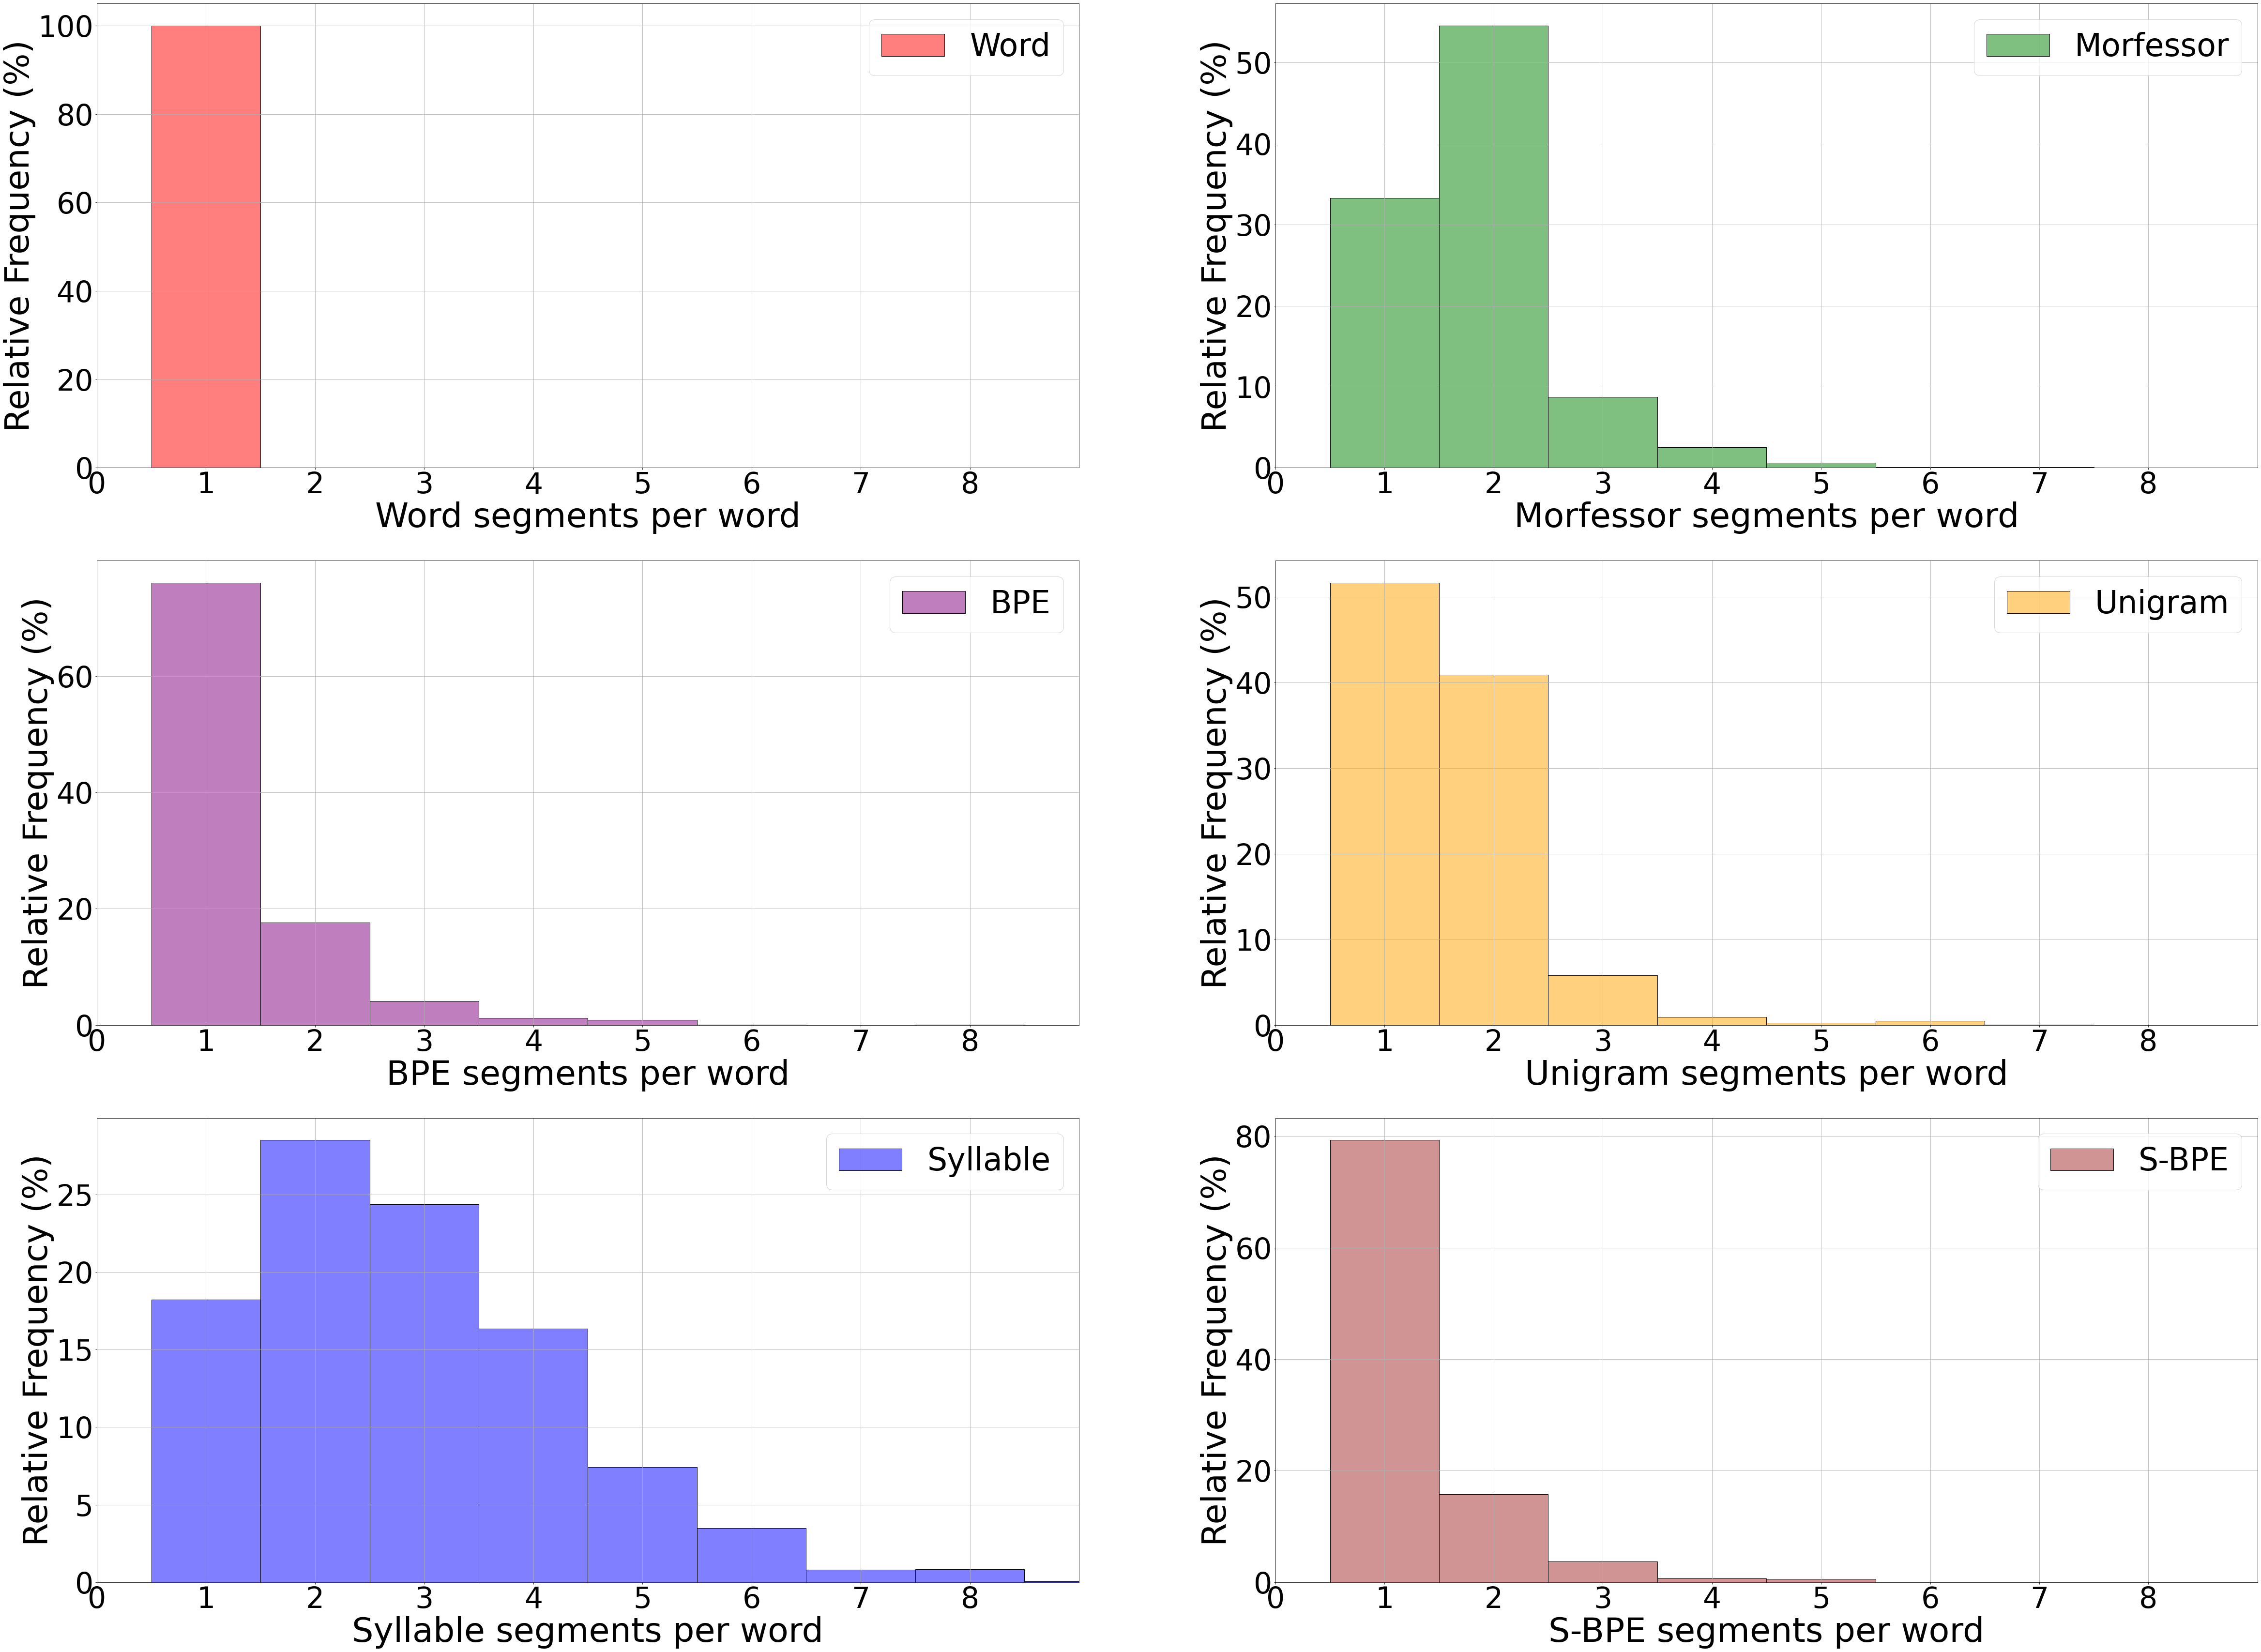
\includegraphics[width=0.95\textwidth]{segmentsperword.png}
    \caption{Distribution of the number of subword segments per word}
    \label{fig:histogram-wordlength}
\end{figure}


The distribution of number of segments per word in the test dataset is
illustrated in Fig. \ref{fig:histogram-wordlength}. Word segmentation does not
beak down the words, resulting in a single bar graph. In BPE, Unigram and S-BPE
segmentation methods, more than 50\% of the words remain unsegmented, followed
by words being segmented into two subwords. In Morfessor segmentation, the
distribution shows more than half the words are segmented into two, followed by
words remaining unsegmented. The percentage of words that get segmented into
more than two segments are rare in all these methods. However in syllable
segmentation, about 28\% and 24\% of words get segmented into two and three
subwords respectively. The segment length per word is more broadly distributed
in syllable segmentation.


\begin{table}[htpb]
    \centering
    \caption{Sentence length statistics in terms of the number of segments per sentence.}
    \label{tab:sentenceseg_stat}
    \begin{tabular}{lccr}
        \hline \hline
        \textbf{Segmentation} & \textbf{Minimum} & \textbf{Maximum} & \textbf{Mean} \\
        \hline
        Word                  & $5$              & $14$             & $6.4$         \\
        BPE                   & $5$              & $26$             & $8.5$         \\
        Morfessor             & $6$              & $29$             & $11.7$        \\
        Unigram               & $5$              & $29$             & $10.1$        \\
        Syllable              & $8$              & $49$             & $19.9$        \\
        S-BPE                 & $5$              & $25$             & $8.1$         \\ \hline
    \end{tabular}

\end{table}

On analysing the segmentation statistics over sentences, we get the values
reported in Table \ref{tab:sentenceseg_stat}. It describes the minimum, maximum
and mean number of segments per sentence. Syllable segmented sentences contain
on an average 19.9 subword segments, which is the highest count of all.
Sentences that contain large number of segments would need longer n-gram
language model context to guide the decoding \cite{SMIT2021101158}. We will
analyse its impact on ASR later in section \ref{sec:Ch-openvocab-analysis}.


\subsubsection{Mean Segment Length}

The \gls{msl}, defined as the average number of characters in a segment, depends on
the segmentation strategy. The distribution of segment lengths, in the form of
box plots is shown in Figure \ref{fig:segmentlength}. The gls{msl} is the highest for
words (8.3) as expected and the smallest is for syllables (2.2). The MSL values
of other segmentation methods are 3.9, 4.3, 4.5 and 4.8 respectively for
Morfessor, Unigram, BPE and S-BPE.

Comparatively smaller box for syllable, indicates the length is distributed
closely about the median value, with very little outliers. However for word
segmentation, the length of box plot is larger, indicating the segment lengths
vary widely.
% The MSL in test datasets is tabulated in Table \ref{tab:meansegmentlength}. 

% \begin{table}[ht]
%     \caption{Mean length of segments}
%     \label{tab:meansegmentlength}
%     \centering
%     \begin{tabular}{lc}
%         \hline \hline
%         \textbf{Segmentation} & \textbf{MSL} \\
%         \hline
%         Word  & 7.1\\
%         S-BPE & 5.5\\ 
%         BPE &  5.3\\
%         Unigram &  4.5\\
%         Morfessor & 3.8 \\
%         Syllable & 2.2\\ \hline
%     \end{tabular}

% \end{table}

% \begin{figure*}[ht]
%     \centering
%     \includegraphics[width=\textwidth]{histogram-segmentlength.png}
%     \caption{Histogram plot of the segment length distribution}
%     \label{histogram-segmentlength}
% \end{figure*}

% A detailed histogram plot of segment length is presented in Figure \ref{histogram-segmentlength}.  

\begin{figure}[htpb]
    \centering
    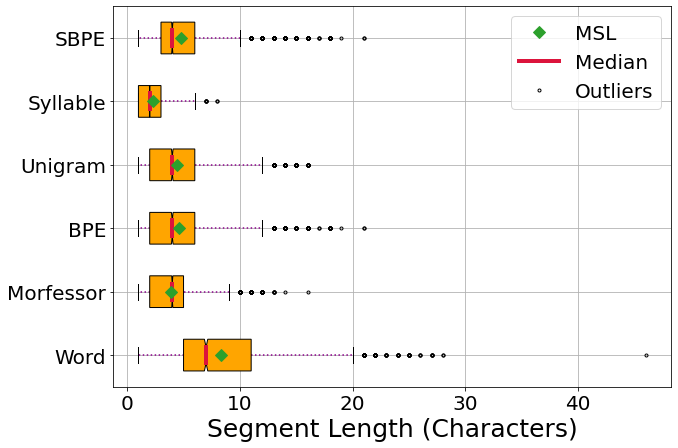
\includegraphics[width=0.85\linewidth]{segmentlength.png}
    \caption{Segment Length distribution in the datasets}
    \label{fig:segmentlength}
\end{figure}

% and longer real time factor to decode [CITATION NEEDED]. 

\subsection{Language modelling Complexity}

The complexity of a language model is related to its difficulty in determining
the next segment from the previous n-gram context. The higher order n-grams
extract more context for the occurrence of a segment and generally reduces
language modelling complexity and hence perplexity. However raising the n-gram
order beyond a limit reintroduces the data sparsity problem, resulting in
unimproved perplexity and SPS values \cite{Mousa1995}. Subword language models
require higher order n-grams to capture the context, than word based ones
\cite{pilar2022subword}. In our experiments we create language models of orders
$n-gram=2$ to $6$ and analyse their complexity in terms of perplexity and SPS.

\begin{table}[ht]
    \centering
    \caption{Language modelling Complexity in terms of Perplexity}
    \label{tab:perplexity}
    \begin{tabular}{l|cccccc}
        \hline \hline
        \textbf{n-gram} & \textbf{Word}                            & \textbf{BPE} & \textbf{Morf.} & \textbf{Uni.} & \textbf{Syl.} & \textbf{S-BPE} \\ \hline

        \hline
                       & \multicolumn{6}{c}{\textbf{Perplexity}}                                                                                  \\ \hline

        $2$            & $2266$                                   & $334$        & $162$          & $287$         & $44$          & $387$          \\ $3$   & $2188$ & $245$ &
        $111$          & $211$                                    & $19$         & $308$                                                           \\ $4$ & $2187$ & $242$ & $107$ & $208$ & $16$ & $307$
        \\ $5$ & $2188$ & $241$ & $107$ & $207$ & $16$ & $307$ \\ $6$ & $2188$ & $242$
                       & $107$                                    & $207$        & $16$           & $307$                                          \\ \hline
        %  \textbf{} & \multicolumn{6}{c|}{\textbf{SPS}}  \\ \hline
        %  n=2&70  & 98 & 99& 99 &124  &96 \\
        % n=3 & 69 & 93& 92 &94 &98  &92  \\
        %  n=4 &69  & 93& 91& 93 &93 &92\\
        % n=5 & 69 &93& 91& 93&92  &92 \\
        % n=6 & 69 & 93 & 91 & 93&92 &92\\
        % \hline

    \end{tabular}

\end{table}

Table \ref{tab:perplexity} presents the values of perplexity over different
segmentation and n-gram orders. For any given n-gram order, it can be observed
from this table that the perplexity value follows the pattern: Word $>$ S-BPE
$>$ BPE > Unigram $>$ Morfessor $>$ Syllable. This is inversely correlated with
the mean number of segments per sentence, $N$, tabulated in Table
\ref{tab:sentenceseg_stat}. Lower the value of $N$, higher is the perplexity.
However the perplexities are not comparable across different segmentation
methods \cite{Mie2016Can}. But for a specific segmentation, the perplexity can
be compared along the variations in n-gram orders. So it can be concluded that
the fourth order syllable level language model with lower perplexity is an
improved model than the corresponding second order language model with higher
perplexity. But it does not necessarily imply the fourth order syllable level
language model with lower perplexity is better than fourth order word level
language model with higher perplexity.
% For any given segmentation method, the best perplexity value occurs for $n\ge4$. 
% The use of subword based models mitigates the detrimental effects of data sparsity by reducing perplexity. 

\begin{table}[ht]
    \centering
    \caption{Language Modelling Complexity in terms of SPS}
    \label{tab:sps}
    \begin{tabular}{l|cccccc}
        \hline \hline
        \textbf{n-gram} & \textbf{Word}                     & \textbf{BPE} & \textbf{Morf.} & \textbf{Uni.} & \textbf{Syl.} & \textbf{S-BPE} \\ \hline

        \textbf{}      & \multicolumn{6}{c}{\textbf{SPS}}                                                                                  \\ \hline
       $2$            & $70$                                & $98$           & $99$             & $99$            & $124$           & $96$             \\
        $3$            & $69$                                & $93$           & $92$             & $94$            & $98$            & $92$             \\
        $4$            & $69$                                & $93$           & $91$             & $93$            & $93$            & $92$             \\
       $5$            & $69$                                & $93$           & $91$             & $93$            & $92$            & $92$             \\
        $6$            & $69$                                & $93$           & $91$             & $93$            & $92$            & $92$             \\
        \hline

    \end{tabular}

\end{table}

% In our experiments we create language models of orders n=2 to 6. 

% \begin{table*}[]
%     \centering
%     \caption{Language modelling Complexity in terms of Perplexity (PPL) and Surprisal per Sentence (SPS) for dataset T1}
%     \label{lmcomplexity}
%     \begin{tabular}{l|ccccc|ccccc}
%         \hline \hline
%         \textbf{Segmentation} & \multicolumn{5}{c|}{\textbf{PPL}} & \multicolumn{5}{c}{\textbf{SPS}} \\
%         \hline
%         &n=2&n=3&n=4&n=5&n=6&n=2&n=3&n=4&n=5&n=6\\ \hline
%         Word&2266.38&2188.43&2187.96&2188.10&2188.10&70.20&69.88&69.88&69.88&69.88 \\
%         BPE&334.05&245.60&242.00&241.97&242.02&98.72&93.49&93.24&93.24&93.24\\
%         Morfessor&162.18&111.01&107.80&107.32&107.38&99.91&92.47&91.90&91.81&91.82 \\
%         Unigram&287.38&211.65&208.17&207.60&207.59&99.50&94.12&93.83&93.78&93.78\\
%         Syllable&44.24&19.65&16.97&16.53&16.44&124.71&98.00&93.19&92.32&92.14\\
%         S-BPE&387.76&308.58&307.10&307.16&307.21&96.43&92.74&92.66&92.66&92.66\\ \hline
%     \end{tabular}

% \end{table*}

The SPS values obtained in our experiments are shown in Table \ref{tab:sps}. As
expected, the SPS reduces initially and then stabilises with increase in n-gram
order for every segmentation method. However, it is interesting to note that
the best set of SPS values are obtained for word segment based language model.
Syllable segments of lower n-gram orders show higher SPS values than all other
segmentation methods. For the test corpus under evaluation, all subword segment
based language models exhibit a comparable SPS value of $\approx 92$, at higher
n-gram orders ($n\ge4$). To conclude, word level language model is better off
than all the segmented language models in terms of SPS. This pattern is
previously observed in \cite{SMIT2021101158}, where the complexity is computed
in terms of $PPL_w(S)$.

The impact of subword segment based language modelling on ASR decoder needs to
be evaluated in terms of its ability to recover OOV words and corresponding
reduction in WER, which is attempted in the following section. However,
lowering the language model complexity does not always ensure an improvement in
automatic speech recognition accuracy
\cite{SMIT2021101158,klosowski2017statistical}.

\subsection{Evaluation of ASR performance}

% \subsubsection{Word Error Rate}
\label{sec:WER}

To begin with, we present the ASR error rate which is computed as WER. It is
based on the number of words inserted, deleted and substituted  in
the predicted speech transcript when compared to the ground truth transcript
according to (\ref{eq:wer2}).
\begin{equation}
	\label{eq:wer2}
	WER = \frac{(Insertions\ +\ Deletions\ +\ Substitutions)\ \times\ 100}{(Number\ of\ words)}
\end{equation}

The evaluation is performed on a multi-speaker studio recorded dataset from the
same domain as the train dataset. About 14\% of words in this test dataset are
OOV words, which can not be recovered by word based ASR. According to
\cite{bisani2005open}, it has been shown that the presence of an OOV word in
test set can result in approximately two errors during ASR decoding.

\begin{figure}[ht]
    \centering
    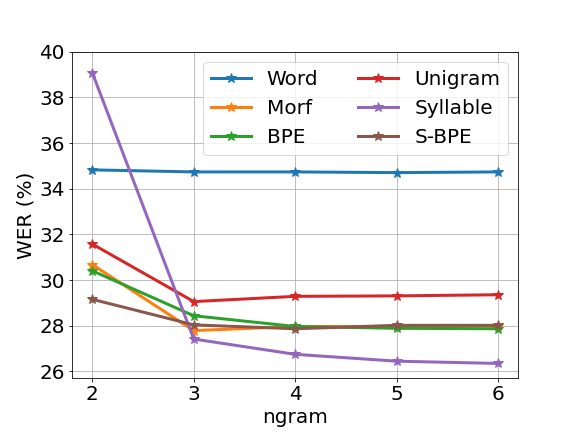
\includegraphics[width=0.8\linewidth]{WER.png}
    \caption{ASR performance evaluation in terms of the WER (lower is better)}
    \label{fig:WER}
\end{figure}

\begin{figure*}[ht]
    \centering
    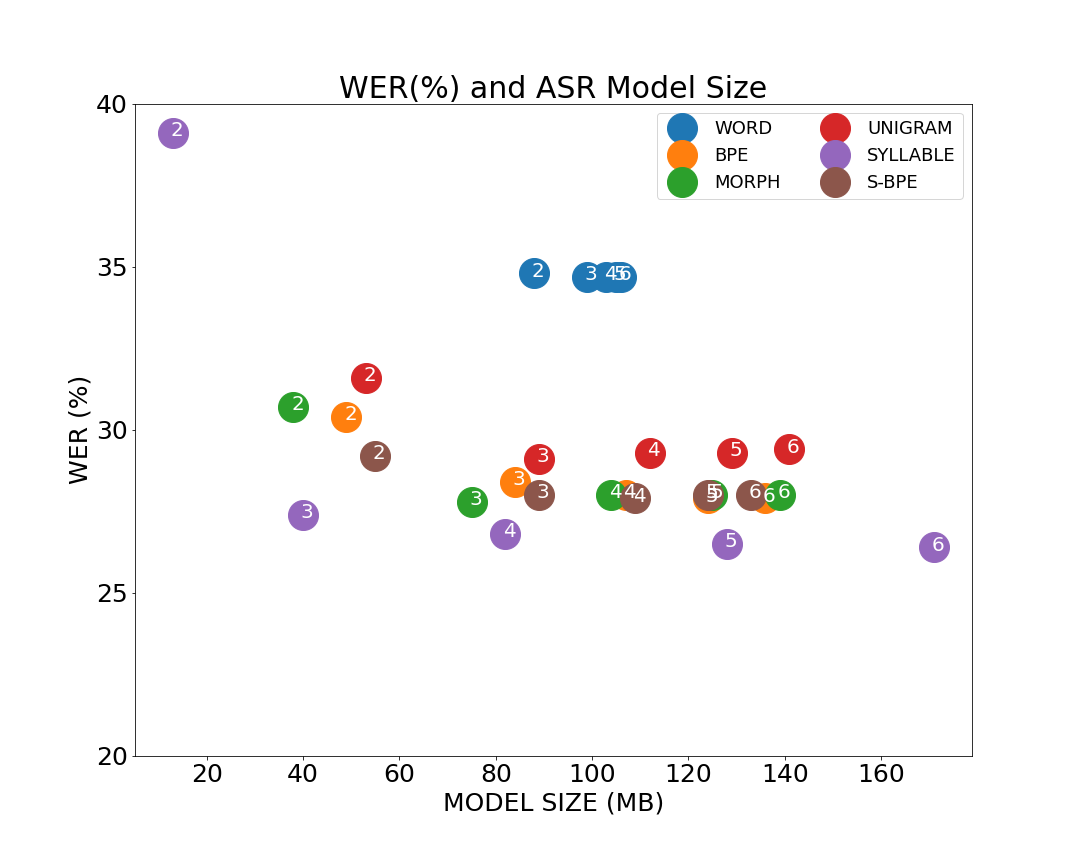
\includegraphics[width=0.9\textwidth]{Size-WER.png}
    \caption{Trade-off between ASR performance and Model Memory Requirement (n-gram order is shown as labels)}
    \label{fig:Size-WER}
\end{figure*}

The WER of different segmentation methods is shown in Fig. \ref{fig:WER}. The
baseline word model with a lexicon size of 79k has a word error rate (WER) of
$\approx$ 35\% for all n-gram orders. The performance of all subword models is
better than the baseline, except for bigram syllable language model. However,
for n-gram orders 3 and above, syllables demonstrate an improvement in WER
compared to all other segmentation methods and n-gram orders. Syllables with the
smallest MSL among all segmentation methods, require more n-gram context to make
a reasonable prediction about the next subword segment. But once it has enough
context, the predictions become more reliable as exemplified in the WER
reduction in Fig. \ref{fig:WER}.

Syllable is the only segmentation method that show consistent improvement in
WER, the best being 26.4\%, at the n-gram order $n=6$. But the relative
improvement diminishes with the n-gram order. For all other segmentation
methods, the WER does not show any improvement beyond n-gram$=4$. The performance
of S-BPE, BPE and Morfessor remains closer at about 28\% WER, for n-gram order
of 4 and beyond. The best WER provided by Unigram segmentation is 29\%.

% \begin{table}[ht]
%     \centering
%     \caption{WER on Test dataset}
%     \label{tab:sps}
%     \begin{tabular}{|l|cccccc|}
%         \hline \hline
%         \textbf{n-gram} & \textbf{Word}&\textbf{BPE}&\textbf{Morf.}&\textbf{Uni.}&\textbf{Syl.}&\textbf{S-BPE}  \\ \hline

%     \textbf{} & \multicolumn{6}{c|}{\textbf{WER}}  \\ \hline

% n=2&34.8 & 30.4 & 30.7 & 31.6 & 39.1 & 29.2 \\
% n=3&\textbf{34.7} & 28.4 & \textbf{27.8} & 29.1 & 27.4 & 28.0 \\
% n=4&34.7 & 28.0 & 28.0 & \textbf{29.3} & 26.8 & \textbf{27.9} \\
% n=5&34.7 & \textbf{27.9} & 28.0 & 29.3 & 26.5 & 28.0 \\
% n=6&34.7 & 27.9 & 28.0 & 29.4 & \textbf{26.4 }& 28.0 \\
%    \hline

%     \end{tabular}

% \end{table}

\subsubsection{WER of OOV Words}
% \begin{figure}[ht]
%     \centering
%     \includegraphics[width=0.9\linewidth]{OOV-WER.png}
%     \caption{WER on OOV words}
%     \label{fig:OOVWER}
% \end{figure}
To study the performance of subword based ASR compared to the baseline word
model on OOV recovery, we compute the WER, specifically for OOV words. The OOV
words in the test set are determined with respect to the word level lexicon.
The results are tabulated in Table \ref{tab:oov-wer}.

\begin{table}[ht]
    \centering
    \caption{WER on OOV words}
    \label{tab:oov-wer}
    \begin{tabular}{rr}
        \hline \hline
        \textbf{Method} & \textbf{OOV-WER(\%)} \\ \hline
        Word            & $100.0$              \\
        Morfessor       & $55.3$               \\
        BPE             & $53.1$               \\
        Unigram         & $55.0$               \\
        Syllable        & $49.9$               \\
        S-BPE           & $50.2$               \\ \hline
        % \textbf{} & \multicolumn{6}{c|}{\textbf{OOv}}  \\ \hline

        \hline

    \end{tabular}

\end{table}

Since OOV words can not be recovered by a word segment based ASR, The OOV-WER
is 100\% for the baseline word based ASR. To analyse the extend of \gls{oovwer} in
subword segmented ASR, we use the \texttt{texterrors} Python
library\cite{braun2021comparison}. The OOV-WER values are computed
corresponding to the best WER values reported in section \ref{sec:WER}.
Providing the list of OOV words in the test set along with the true speech
transcripts, this library computes the OOV-WER of the subword ASR model. The
syllable segments perform the best, which has reduced the OOV-WER to 49.9\%,
closely followed by S-BPE segments. Purely data driven segmentation techniques
of BPE, Morfessor and Unigram could also recover the OOV words, but the WER are
not as promising as the Syllable and S-BPE segments.

% \subsubsection{OOV- CER}
% % \begin{figure}[ht]
% %     \centering
% %     \includegraphics[width=0.9\linewidth]{OOV-CER.png}
% %     \caption{CER on OOV words}
% %     \label{fig:OOVCER}
% % \end{figure}

% \begin{table}[ht]
%     \centering
%     \caption{WER on OOV words}
%     \label{tab:oov-wer}
%     \begin{tabular}{|l|cccccc|}
%         \hline \hline
%         & \textbf{Word}&\textbf{BPE}&\textbf{Morf.}&\textbf{Uni.}&\textbf{Syl.}&\textbf{S-BPE}  \\ \hline

%  OOV-CER &90.7 & 47.1& 49.5 & 51.4 & 44.4 & 54.8 \\ \hline

%     % \textbf{} & \multicolumn{6}{c|}{\textbf{OOv}}  \\ \hline

%    \hline

%     \end{tabular}

% \end{table}
% Character Error rate of OOV words 
\subsubsection{Trade-off between WER and Model Memory Requirement}

The order of n-gram impacts the memory requirement of the ASR model. To study
the the model memory requirement, we compute the size of weighted FST graph
(\textit{HCLG.fst}) used for decoding. In the trade-off diagram shown in Fig.
\ref{fig:Size-WER}, the model size of the word based baseline ASR model does
not change significantly with the n-gram order. However, the error rate of the
word-based baseline model is higher than all subword-based models, except for
the syllable bigram ASR. Although the syllable bigram ASR has the smallest
model size, its error rate is so high that it is not practical to use and is
therefore not considered in further analysis.

For lower-order language models ($n\le4$), the subword-segmented ASR models
have significantly smaller sizes compared to the word-based models, while also
having a lower error rate. Syllable segments require less memory at smaller
n-gram orders, but the model size increases quickly with the increase in n-gram
order, while the corresponding reduction in error rate is relatively small.
From the figures \ref{fig:WER} and \ref{fig:Size-WER}, it can be seen that the
4-gram syllable language model, which has a better error rate than all other
subword-segmented models, has the smallest model size. \vspace{-0.4cm}
\subsection{Comparison with Other Reported works}

Since the previously published work on subword ASR for Malayalam
\cite{sreeja-hybrid-2022}, was tested on a private dataset, the comparison of
results is not meaningful and hence not attempted. The current study is a
detailed expansion of the experiments reported in \cite{mlphon2022kavya}, with the difference that graphemic lexicons are used instead of phonemic ones, focusing on a medium OOV test
dataset where the WER improvement is notable and within a reasonable rage.

\section{Findings and Discussions}
\label{sec:Ch-openvocab-analysis}

In this section we analyse the experimental results to draw the relationship
between segmentation methods and language modelling and their impact on ASR.

\subsection{Language modelling Complexity }

To compare language modelling performance across different segmentation
methods, we use the SPS metric \cite{Mie2016Can}. The major observations are listed below:

\begin{enumerate}
    \item For all segmentation methods,
language modelling complexity decreases with n-gram order initially, and then
stabilises. 

\item Raising the n-gram order
beyond a limit (different for different segmentation methods) reintroduces the data sparsity problem, resulting in unimproved
perplexity values \cite{Mousa1995}. This limit is 3 for words, BPE and S-BPE, 4 for Morfessor and Unigram and 5 for syllables as presented in Table \ref{tab:sps}.

\item In terms of SPS, the language modelling complexity is the least for words than all other
segmentation methods.

\item The lower LM complexity in terms of SPS does not guarantee improved WER \cite{SMIT2021101158}.


\end{enumerate}

%  It can be concluded that creating language
% models of orders higher than 3 for , does not bring in any advantage in terms of
% complexity reduction, as read from Table \ref{tab:sps}. It can also be observed
% that,  However it is worth noting that the best
% language model, need not always provide the best speech recognition results
% .

\subsection{ASR results}

Syllable segments give the best WER among all other segmentation strategies,
and it happens for n-gram orders 3 and above. It could recover more than 50\% of
the OOV words correctly. This performance improvement can not unambiguously be
attributed to the segmentation happening at valid orthographic boundaries. The
proposed S-BPE segmentation did not bring in much reduction in WER, and has a
performance similar to that of BPE and Morfessor segmentation methods and
better than word and Unigram segmentation.

The WER result obtained for Malayalam ASR is not correlated with the language
modelling complexity of the segmentation method. This pattern was previously
observed and reported in \cite{SMIT2021101158} for Finnish, Swedish and Arabic
ASR where word segments show least language modelling complexity but the
highest WER. 

The subword lexicons used in our experiments were derived from the word lexicon used in our baseline experiments by the procedure explained in section \ref{sec:ch-openvocab-graphemiclexicon}. In our experiments, we compared various segmentation methods in terms of their lexicon size and WER. The Unigram segmentation method produced the largest subword lexicon, with approximately $19k$ entries, but it also yielded the highest WER of 29\%. On the other hand, the BPE, S-BPE and Morfessor segmentation methods resulted in lexicons with around $10k$ to $15k$ entries and a similar WER of approximately 28\%. However, the syllable segmentation method with the smallest lexicon size of about $6k$ entries had the best WER of 26\%. Overall, our results suggest that smaller lexicon sizes can result in better WERs, when the subword lexicons are derived from a common pool of words. 


An optimal choice of n-gram order helps to build ASR models for memory
constrained environments while maintaining a good recognition accuracy.
Syllable segments with n-gram orders 3 and 4 prove to provide best WER at the
lowest reported model memory requirement.

% The language modelling complexity reported in Tables \ref{tab:perplexity} and \ref{tab:sps} and WER reported in Fig. \ref{fig:WER} are not correlated. When looking at the performance of an ASR system in terms of its WER, the complexity of the language model used by the system is not the only factor that affects its performance. Other factors, such as the relative weight given to the acoustic model and the word insertion penalty used during lattice search, can also influence the WER.  This pattern was previously observed and reported in an open vocabulary speech recognition experiment on Finnish, Swedish, English and Arabic \cite{SMIT2021101158}.

\section{Summary}

The  study presented in this chapter is the first investigation on the diverse aspects of improving speech recognition system in the morphologically complex Malayalam language using subword language modelling techniques. We have presented the detailed investigation of the usage of different subword segmentation strategies to build statistical n-gram language models for usage in hybrid ASR task. The language modelling complexity is evaluated using perplexity and surprisal. We build graphemic pronunciation lexicons of these subword segments. The ASR decoders built by combining these language models and lexicons with a common acoustic model are used to evaluate a multi speaker Malayalam speech dataset having 14\% of OOV words with respect to the baseline word pronunciation lexicon. The ASR performance is evaluated based on the WER, OOV-WER and the model memory requirement. 

It has been demonstrated that the linguistically informed syllable segments perform exceptionally well with a 26\% WER, which is an 8\% improvement from the baseline word level ASR. The hybrid segmentation strategy proposed in this paper, S-BPE reports a WER of 28\%, but it could not beat the syllable subword segments in terms of WER. 

To conclude, the syllable subword segments have the advantage of requiring less memory for the model, especially at n-gram orders of 3 and 4, while still maintaining a low error rate. Syllable subwords also have the lowest error rate for out of vocabulary words, showing that they are effective at correctly identifying about half of these words. Overall, syllable segmentation provides benefits in terms of reduced model memory requirements and a lower error rate, despite having higher language modelling complexity compared to word-based language models.
